% single_phase_grid_tied_inverter_analysis.tex
% Single-phase grid-tied T-type inverter: plant model, virtual-dq current control on the fundamental of the
% current (first harmonic tracker), single-phase PLL with virtual quadrature, DC-link voltage loop and three-level
% modulation, as implemented in afe_sp_ttype_ctrl_pwm of the library block afe_single_phase_ttype, with the exact
% stationary-frame analysis of the current loop and the discrete implementation operation by operation.
% pwr-control template (AAA_template_latex_settings); numbers and figures: single_phase_grid_tied_inverter_analysis.py
% (python3, numpy, scipy, matplotlib). Compile: pdflatex single_phase_grid_tied_inverter_analysis.tex (twice).
% Rev. 00 - June 2020 - first issue (single_phase_inverter.tex: three control strategies compared)
% Rev. 01 - October 2026 - rewritten for the T-type AFE block of the library
\documentclass[10pt,a4paper]{scrartcl}
\ifdefined\PWRCONTROLSETTINGSLOADED
\endinput
\fi
\def\PWRCONTROLSETTINGSLOADED{1}
% ===================== PACKAGES =====================
\usepackage[british]{babel}
\usepackage[tmargin=1in, bmargin=1in, lmargin=0.75in, rmargin=0.75in]{geometry}
\usepackage[dvipsnames,table]{xcolor}  % prima di tikz, listings, ecc.

\usepackage{tikz}
\usepackage{graphicx}
\usepackage{pgfplots}
\pgfplotsset{width=12cm, compat=1.9}
\usepackage{setspace}
\usepackage{chemmacros}
\usepackage{chemfig}
\usepackage{tabularray}
\usepackage{makeidx}
\usepackage{epstopdf}
\usepackage{amssymb}
\usepackage{mathrsfs}
\usepackage{bm}
\usepackage{amsmath}
% esint deve essere caricato DOPO amsmath: entrambi definiscono \iint, \iiint,
% \iiiint e \idotsint. Le si rende indefinite in modo che esint le ridefinisca
% (versioni con i simboli di integrale multiplo corretti) senza errori.
\let\iint\undefined
\let\iiint\undefined
\let\iiiint\undefined
\let\idotsint\undefined
\usepackage{esint}
\usepackage{enumitem}
%\usepackage[english]{varioref}
\usepackage{physics}
\usepackage{lipsum}
\usepackage{fancyhdr}
\usepackage{float}
\usepackage{empheq}
\usepackage[framemethod=tikz]{mdframed}
\numberwithin{equation}{section}
\usepackage{eso-pic}
\usepackage{calc}
\usepackage{nccmath}
\usepackage{caption}
\usepackage{subcaption}
\usepackage{gensymb}
\usepackage{amsfonts, amsthm, epsfig, epstopdf, titling, url, array}
\usepackage{tabularx}
\usepackage{makecell}
\usepackage{booktabs}
\usepackage{array}
\usepackage{siunitx}
\sisetup{input-digits=0123456789\pi}
\usepackage[symbol]{footmisc}
\usepackage{multicol}
%\usepackage{boondox-cal}
\usepackage{blindtext}
\usepackage{changepage}
\usepackage{nomencl}
\usepackage{hyperref}
\usepackage{xurl}
\usepackage{ragged2e}
\usepackage[version=4]{mhchem}  % ← conflitto di opzioni
\usepackage{longtable}
\usepackage{chemformula}
\usetikzlibrary{arrows.meta,positioning,calc}
\usepackage[page,toc]{appendix}


% ===================== SI UNITS =====================
\DeclareSIUnit\atm{atm}
\DeclareSIUnit{\var}{var}
\DeclareSIUnit{\pu}{p.u.}
\sisetup{detect-weight=true, detect-inline-weight=math}

% ===================== MATH OPERATORS =====================
%\DeclareMathOperator{\rank}{rank}
\DeclareMathOperator{\atantwo}{atan2}
\DeclareMathOperator{\spn}{span}

% ===================== COMMANDS =====================
%\newcommand{\abs}[1]{\left|#1\right|}
\newcommand{\sign}{\text{sign}}
\newcommand{\centered}[1]{\begin{tabular}{@{}l@{}} #1 \end{tabular}}

% ===================== COLORS =====================
\definecolor{mycolor1}{rgb}{0.97, 0.97, 0.97}
\definecolor{mycolor2}{rgb}{0.97, 0.97, 0.97}
\definecolor{tableShade}{gray}{0.9}

% ===================== THEOREM ENVIRONMENTS =====================
\theoremstyle{it}
\newtheorem{defn}{Definition}[section]
\newtheorem{assumption}{Assumption}[section]
\newtheorem{thm}{Theorem}[section]
\newtheorem{lemma}{Lemma}[section]
\newtheorem{corollary}{Corollary}[section]
\theoremstyle{definition}
\newtheorem{example}{Example}[section]

% ===================== CUSTOM ENVIRONMENTS =====================
\newenvironment{myitemize_1}{
	\begin{itemize}[topsep=0pt]
		\setlength{\topsep}{2pt}
		\setlength{\itemsep}{2pt}
		\setlength{\parskip}{2pt}
		\setlength{\parsep}{2pt}
	}{\end{itemize}}

\newmdenv[
innerlinewidth=0.5pt,
roundcorner=4pt,
backgroundcolor=mycolor2,
linecolor=mycolor1,
innerleftmargin=6pt,
innerrightmargin=6pt,
innertopmargin=6pt,
innerbottommargin=6pt
]{mybox}

% ===================== TABLE COLUMN TYPES =====================
\newcolumntype{Y}{>{\hsize=2\hsize}X}
\newcolumntype{Z}{>{\centering\arraybackslash\hsize=0.857\hsize}X}

% ===================== SECTION DEPTH =====================
\setcounter{secnumdepth}{3}
\setcounter{tocdepth}{3}

% ===================== PAGE STYLE =====================
\setlength{\headheight}{20pt}
\setlength{\headsep}{20pt}

\pagestyle{fancy}
\fancypagestyle{firstpage}{\rhead{}}
\fancyhead[L]{\slshape\nouppercase{\leftmark}}
\chead{}
\rhead{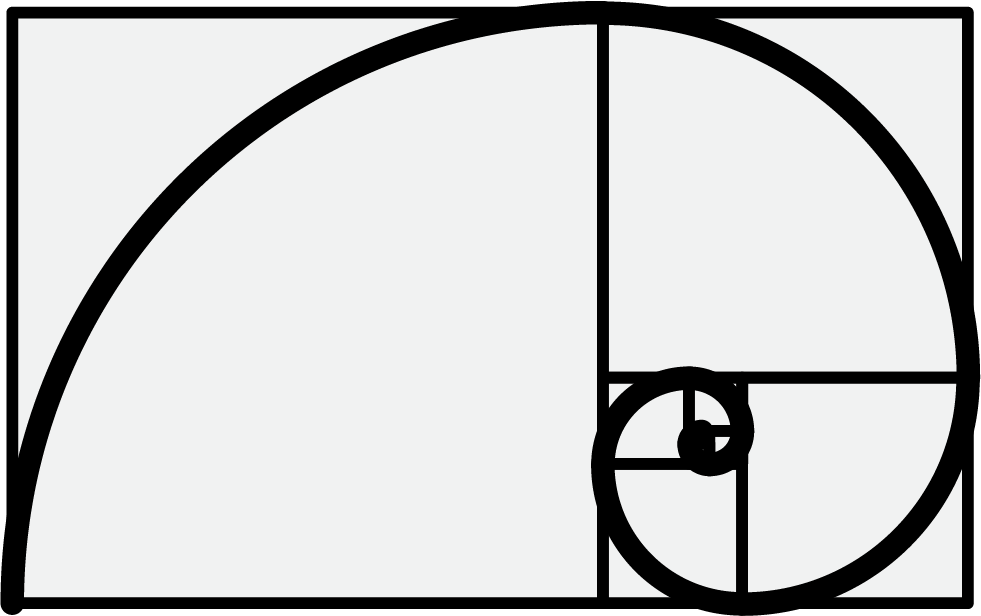
\includegraphics[height=0.75cm]{../../AAA_template_latex_settings/pwr-control_logo_doc.png}}
\lfoot{\href{https://github.com/pwr-control}{\color{black} pwr-control}}
\cfoot{-\ \thepage\ -}
\rfoot{\textit{}}
\renewcommand{\headrulewidth}{0.4pt}
\renewcommand{\footrulewidth}{0.4pt}


\geometry{
	a4paper,
	top    = 2.5cm,
	bottom = 3.0cm,
	left   = 2.5cm,
	right  = 2.5cm
}

\hypersetup{
	colorlinks = true,
	urlcolor   = blue,
	linkcolor  = black,
	citecolor  = black
}

\pagenumbering{gobble}


\rfoot{\small Rev.~01}
\geometry{left=2.0cm, right=2.0cm}
\usepackage{circuitikz}
\usetikzlibrary{shapes.geometric}
\newcolumntype{R}[1]{>{\RaggedRight\arraybackslash}p{#1}}

\sisetup{per-mode=symbol,range-phrase={\text{--}},range-units=single}
\setlist{nosep}
\setlength{\parindent}{0pt}
\setlength{\parskip}{3pt}
\allowdisplaybreaks

% --- shorthand ---
\newcommand{\ts}{t_s}
\newcommand{\tc}{t_c}
\newcommand{\wo}{\omega_0}
\newcommand{\wres}{\omega_{res}}
\newcommand{\fres}{f_{res}}
\newcommand{\kmod}{k_{mod}}
\newcommand{\kpi}{k_{p,i}}
\newcommand{\kii}{k_{i,i}}
\newcommand{\kpu}{k_{p,u}}
\newcommand{\kiu}{k_{i,u}}
\newcommand{\jj}{\mathrm{j}}
\newcommand{\ee}{\mathrm{e}}
\newcommand{\dif}{\mathrm{d}}
\newcommand{\pu}{\,\mathrm{pu}}
\newcommand{\code}[1]{\texttt{#1}}
\newcommand{\ihat}{\hat{\imath}}
\newcommand{\Ceq}{C_{eq}}
\newcommand{\Hu}{H_u}
\newcommand{\Hv}{H_v}
\renewcommand{\Re}{\operatorname{Re}}
\renewcommand{\Im}{\operatorname{Im}}

% =============================================================
%  DOCUMENT DATA (title page: AAA_template_latex_settings/titlepage.tex)
% =============================================================
\newcommand{\DocCategory}{Technical Note}
\newcommand{\DocField}{Power Electronics and Control Systems}
\newcommand{\DocTitle}{%
	{\fontsize{20}{24}\selectfont\bfseries Single-Phase Grid-Tied T-Type Inverter:} \\[12pt]
	{\fontsize{16}{26}\selectfont\bfseries model, control design \\[8pt] and discrete implementation}
}
\newcommand{\DocSubtitle}{The controller of the library block \texttt{afe\_single\_phase\_ttype} (\texttt{afe\_sp\_ttype\_ctrl\_pwm}): \\[6pt] virtual-dq current loop on the fundamental of the current, single-phase PLL, \\[6pt] DC-link voltage loop and three-level modulation}
\newcommand{\DocAuthor}{Davide Bagnara}
\newcommand{\DocRevision}{01}
\newcommand{\DocDate}{October 2026}
\newcommand{\DocAbstract}{%
This note documents the control of the single-phase three-level T-type grid-tied inverter implemented in the MATLAB Function \texttt{afe\_sp\_ttype\_ctrl\_pwm} of the library block \texttt{afe\_single\_phase\_ttype}, the AC module of the solid-state-transformer test bench (\SI{50}{kW}, \SI{800}{V} DC link, one phase of a \SI{690}{V} system, \SI{4}{kHz} double update). The converter has a single physical current: a first harmonic tracker estimates its fundamental and the quadrature of the fundamental, the pair is regulated by a vector PI in the dq frame of a single-phase PLL, with the DC-link feed-forward, and the modulation vector is projected back on the single axis. The note gives the plant model (LCL resonance at \SI{1.4}{kHz}, above $f_s/6$), the control structure block by block and an analysis of the current loop that is exact for the single-phase case: with a locked PLL the loop is the stationary-frame controller $\Ceq(s) = \kpi\Hu + \kii\,(s\Hu - \wo\Hv)/(s^2 + \wo^2)$, a proportional-resonant controller shaped by the two outputs of the tracker. The tracker gain-stabilizes the filter resonance but leaks a DC input into both outputs, so that the controller has the DC gain $0.75\kpi - 1.24\kii/\wo$, negative for $\kii/\kpi > \SI{190}{rad/s}$: the library default ($\kpi = 0.1$, $\kii = \SI{20}{s^{-1}}$) leaves a marginally unstable DC mode and $\kpi = 0.15$ is recommended (crossover \SI{112}{Hz}, phase margin \SI{44}{\degree}, DC pole \SI{-30}{s^{-1}}). The PLL is shown to be a SOGI-QSG with $k = 0.5$ followed by a type-1 loop and an angle observer; the DC-link loop (\SI{8}{Hz}, moving average over one grid period), the three-level modulator and the discrete implementation are reviewed in the same way. A companion Python script reproduces every number and figure with a sampled-data simulation of the controller as coded.
}
\newcommand{\RevisionHistory}{%
	00 & June 2020 & First issue: three current control strategies compared. & \DocAuthor \\
	01 & October 2026 & Rewritten for the T-type AFE block of the library. & \DocAuthor \\
}
\newcommand{\MetaLabelA}{Project Repository}
\newcommand{\MetaValueAUrl}{https://github.com/pwr-control/library.git}
\newcommand{\MetaValueALabel}{library.git (masked\_models/afe\_single\_phase\_ttype)}
\newcommand{\MetaLabelB}{Framework}
\newcommand{\MetaValueB}{MATLAB/Simulink/Simscape; Python 3 (companion script)}

\begin{document}
% =============================================================
%  pwr-control LaTeX template - FRONTESPIZIO
%
%  Da richiamare come prima istruzione dopo \begin{document}:
%      % =============================================================
%  pwr-control LaTeX template - FRONTESPIZIO
%
%  Da richiamare come prima istruzione dopo \begin{document}:
%      % =============================================================
%  pwr-control LaTeX template - FRONTESPIZIO
%
%  Da richiamare come prima istruzione dopo \begin{document}:
%      \input{../../AAA_template_latex_settings/titlepage}
%
%  Il documento deve definire prima di \begin{document}:
%      \DocCategory   categoria del documento
%      \DocField      area tecnica
%      \DocTitle      titolo (una o due righe)
%      \DocSubtitle   sottotitolo
%      \DocAuthor     autore/i, separati da virgola
%      \DocRevision   numero di revisione corrente (es. 00)
%      \DocDate       data della revisione corrente
%      \DocAbstract   abstract
%      \RevisionHistory  righe della tabella di revisione, nel formato
%                        Rev. & Date & Description & Authors \\
%      \MetaLabelA \MetaValueAUrl \MetaValueALabel
%      \MetaLabelB \MetaValueB
% =============================================================

\providecommand{\DocCategory}{Technical Research Report}
\providecommand{\DocField}{Power Electronics and Control Systems}
\providecommand{\DocSubtitle}{}
\providecommand{\DocRevision}{00}
\providecommand{\DocAbstract}{}
\providecommand{\RevisionHistory}{%
	\DocRevision & \DocDate & First issue. & \DocAuthor \\
}

\titlepage

% ---- Intestazione centrata ----
\begin{center}
	{\Large\scshape \DocCategory}\\[8pt]
	{\large\scshape \DocField}
\end{center}

\vspace{30pt plus 4pt minus 14pt}
\noindent\rule{\linewidth}{0.8pt}

% ---- Titolo ----
\begin{center}
	\DocTitle
\end{center}

\vspace{4pt}
\noindent\rule{\linewidth}{2.2pt}

% ---- Sottotitolo ----
\begin{center}
	\begin{onehalfspace}
		{\large\itshape \DocSubtitle}
	\end{onehalfspace}
\end{center}

% ---- Authors / Revision / Date ----
\vspace{30pt plus 4pt minus 14pt}

\noindent
\begin{minipage}[t]{0.46\linewidth}
	\raggedright
	\textbf{Authors:}\\[2pt]
	\DocAuthor
\end{minipage}%
\hfill
\begin{minipage}[t]{0.22\linewidth}
	\centering
	\textbf{Revision:}\\[2pt]
	\DocRevision
\end{minipage}%
\hfill
\begin{minipage}[t]{0.30\linewidth}
	\raggedleft
	\textbf{Date:}\\[2pt]
	\DocDate
\end{minipage}

\vspace{10pt}
\noindent\rule{\linewidth}{0.8pt}

% ---- Abstract ----
\vspace{24pt plus 4pt minus 12pt}

\begin{center}
	\begin{minipage}{0.88\linewidth}
		\footnotesize
		\begin{onehalfspace}
			\textbf{Abstract:} \DocAbstract
		\end{onehalfspace}
	\end{minipage}
\end{center}

\vfill

% ---- Revision history ----
\begin{center}
	\begin{minipage}{0.96\linewidth}
		\centering
		{\footnotesize\scshape Revision history}\\[6pt]
		{\footnotesize
			\begin{tabular}{@{}cl>{\raggedright\arraybackslash}p{0.36\linewidth}>{\raggedright\arraybackslash}p{0.28\linewidth}@{}}
				\toprule
				\textbf{Rev.} & \textbf{Date} & \textbf{Description} & \textbf{Authors} \\
				\midrule
				\RevisionHistory
				\bottomrule
			\end{tabular}}
	\end{minipage}
\end{center}

\vspace{18pt plus 4pt minus 10pt}

% ---- Metadati in fondo ----
\noindent
\begin{tabular}{@{} r @{\quad} l @{}}
	\textsc{\MetaLabelA:} & {\href{\MetaValueAUrl}{\MetaValueALabel}} \\[3pt]
	\textsc{\MetaLabelB:} & {\MetaValueB}       \\[3pt]
\end{tabular}

% =============================================================
%  Fine frontespizio
% =============================================================
\newpage
\pagenumbering{arabic}
\setcounter{page}{1}

%
%  Il documento deve definire prima di \begin{document}:
%      \DocCategory   categoria del documento
%      \DocField      area tecnica
%      \DocTitle      titolo (una o due righe)
%      \DocSubtitle   sottotitolo
%      \DocAuthor     autore/i, separati da virgola
%      \DocRevision   numero di revisione corrente (es. 00)
%      \DocDate       data della revisione corrente
%      \DocAbstract   abstract
%      \RevisionHistory  righe della tabella di revisione, nel formato
%                        Rev. & Date & Description & Authors \\
%      \MetaLabelA \MetaValueAUrl \MetaValueALabel
%      \MetaLabelB \MetaValueB
% =============================================================

\providecommand{\DocCategory}{Technical Research Report}
\providecommand{\DocField}{Power Electronics and Control Systems}
\providecommand{\DocSubtitle}{}
\providecommand{\DocRevision}{00}
\providecommand{\DocAbstract}{}
\providecommand{\RevisionHistory}{%
	\DocRevision & \DocDate & First issue. & \DocAuthor \\
}

\titlepage

% ---- Intestazione centrata ----
\begin{center}
	{\Large\scshape \DocCategory}\\[8pt]
	{\large\scshape \DocField}
\end{center}

\vspace{30pt plus 4pt minus 14pt}
\noindent\rule{\linewidth}{0.8pt}

% ---- Titolo ----
\begin{center}
	\DocTitle
\end{center}

\vspace{4pt}
\noindent\rule{\linewidth}{2.2pt}

% ---- Sottotitolo ----
\begin{center}
	\begin{onehalfspace}
		{\large\itshape \DocSubtitle}
	\end{onehalfspace}
\end{center}

% ---- Authors / Revision / Date ----
\vspace{30pt plus 4pt minus 14pt}

\noindent
\begin{minipage}[t]{0.46\linewidth}
	\raggedright
	\textbf{Authors:}\\[2pt]
	\DocAuthor
\end{minipage}%
\hfill
\begin{minipage}[t]{0.22\linewidth}
	\centering
	\textbf{Revision:}\\[2pt]
	\DocRevision
\end{minipage}%
\hfill
\begin{minipage}[t]{0.30\linewidth}
	\raggedleft
	\textbf{Date:}\\[2pt]
	\DocDate
\end{minipage}

\vspace{10pt}
\noindent\rule{\linewidth}{0.8pt}

% ---- Abstract ----
\vspace{24pt plus 4pt minus 12pt}

\begin{center}
	\begin{minipage}{0.88\linewidth}
		\footnotesize
		\begin{onehalfspace}
			\textbf{Abstract:} \DocAbstract
		\end{onehalfspace}
	\end{minipage}
\end{center}

\vfill

% ---- Revision history ----
\begin{center}
	\begin{minipage}{0.96\linewidth}
		\centering
		{\footnotesize\scshape Revision history}\\[6pt]
		{\footnotesize
			\begin{tabular}{@{}cl>{\raggedright\arraybackslash}p{0.36\linewidth}>{\raggedright\arraybackslash}p{0.28\linewidth}@{}}
				\toprule
				\textbf{Rev.} & \textbf{Date} & \textbf{Description} & \textbf{Authors} \\
				\midrule
				\RevisionHistory
				\bottomrule
			\end{tabular}}
	\end{minipage}
\end{center}

\vspace{18pt plus 4pt minus 10pt}

% ---- Metadati in fondo ----
\noindent
\begin{tabular}{@{} r @{\quad} l @{}}
	\textsc{\MetaLabelA:} & {\href{\MetaValueAUrl}{\MetaValueALabel}} \\[3pt]
	\textsc{\MetaLabelB:} & {\MetaValueB}       \\[3pt]
\end{tabular}

% =============================================================
%  Fine frontespizio
% =============================================================
\newpage
\pagenumbering{arabic}
\setcounter{page}{1}

%
%  Il documento deve definire prima di \begin{document}:
%      \DocCategory   categoria del documento
%      \DocField      area tecnica
%      \DocTitle      titolo (una o due righe)
%      \DocSubtitle   sottotitolo
%      \DocAuthor     autore/i, separati da virgola
%      \DocRevision   numero di revisione corrente (es. 00)
%      \DocDate       data della revisione corrente
%      \DocAbstract   abstract
%      \RevisionHistory  righe della tabella di revisione, nel formato
%                        Rev. & Date & Description & Authors \\
%      \MetaLabelA \MetaValueAUrl \MetaValueALabel
%      \MetaLabelB \MetaValueB
% =============================================================

\providecommand{\DocCategory}{Technical Research Report}
\providecommand{\DocField}{Power Electronics and Control Systems}
\providecommand{\DocSubtitle}{}
\providecommand{\DocRevision}{00}
\providecommand{\DocAbstract}{}
\providecommand{\RevisionHistory}{%
	\DocRevision & \DocDate & First issue. & \DocAuthor \\
}

\titlepage

% ---- Intestazione centrata ----
\begin{center}
	{\Large\scshape \DocCategory}\\[8pt]
	{\large\scshape \DocField}
\end{center}

\vspace{30pt plus 4pt minus 14pt}
\noindent\rule{\linewidth}{0.8pt}

% ---- Titolo ----
\begin{center}
	\DocTitle
\end{center}

\vspace{4pt}
\noindent\rule{\linewidth}{2.2pt}

% ---- Sottotitolo ----
\begin{center}
	\begin{onehalfspace}
		{\large\itshape \DocSubtitle}
	\end{onehalfspace}
\end{center}

% ---- Authors / Revision / Date ----
\vspace{30pt plus 4pt minus 14pt}

\noindent
\begin{minipage}[t]{0.46\linewidth}
	\raggedright
	\textbf{Authors:}\\[2pt]
	\DocAuthor
\end{minipage}%
\hfill
\begin{minipage}[t]{0.22\linewidth}
	\centering
	\textbf{Revision:}\\[2pt]
	\DocRevision
\end{minipage}%
\hfill
\begin{minipage}[t]{0.30\linewidth}
	\raggedleft
	\textbf{Date:}\\[2pt]
	\DocDate
\end{minipage}

\vspace{10pt}
\noindent\rule{\linewidth}{0.8pt}

% ---- Abstract ----
\vspace{24pt plus 4pt minus 12pt}

\begin{center}
	\begin{minipage}{0.88\linewidth}
		\footnotesize
		\begin{onehalfspace}
			\textbf{Abstract:} \DocAbstract
		\end{onehalfspace}
	\end{minipage}
\end{center}

\vfill

% ---- Revision history ----
\begin{center}
	\begin{minipage}{0.96\linewidth}
		\centering
		{\footnotesize\scshape Revision history}\\[6pt]
		{\footnotesize
			\begin{tabular}{@{}cl>{\raggedright\arraybackslash}p{0.36\linewidth}>{\raggedright\arraybackslash}p{0.28\linewidth}@{}}
				\toprule
				\textbf{Rev.} & \textbf{Date} & \textbf{Description} & \textbf{Authors} \\
				\midrule
				\RevisionHistory
				\bottomrule
			\end{tabular}}
	\end{minipage}
\end{center}

\vspace{18pt plus 4pt minus 10pt}

% ---- Metadati in fondo ----
\noindent
\begin{tabular}{@{} r @{\quad} l @{}}
	\textsc{\MetaLabelA:} & {\href{\MetaValueAUrl}{\MetaValueALabel}} \\[3pt]
	\textsc{\MetaLabelB:} & {\MetaValueB}       \\[3pt]
\end{tabular}

% =============================================================
%  Fine frontespizio
% =============================================================
\newpage
\pagenumbering{arabic}
\setcounter{page}{1}

\tableofcontents
\newpage
\begin{onehalfspace}

% =====================================================================================================
\section{Scope}
\label{sec:scope}

The converter considered here is a single-phase three-level T-type voltage-source inverter with an LC output filter, connected to one phase of a three-phase grid through a line inductance: the AC module of the solid-state transformer (SST) test bench, where two modules in series on one line share the phase voltage of a \SI{690}{V} system and each is fed on its DC link by a CLLC DC transformer. The control is implemented in the MATLAB Function \code{afe\_sp\_ttype\_ctrl\_pwm} of the library block \code{afe\_single\_phase\_ttype} (model \path{afe_single_phase_ttype_mod1}, folder \path{library/masked_models/afe_single_phase_ttype}), which holds the acquisitions, the single-phase PLL, the current loop, the DC-link voltage loop and the three-level PWM of one converter in one block, with a master/slave mode for modules in series; the power stage is the Simscape component \path{afe_ttype_ssc.afe_single_phase_ttype} (\path{library/foundation/pwr_electronics/+afe_ttype_ssc}). The block is used by the bench model \code{sst\_cllc\_ttype\_inv.slx} of the solid-state-transformers repository (folder \path{sst_based_on_full_bridge_ttype_inverter/sst_single_phase_cllc_single_phase_ttype_inv}, parameters in \code{private/sst\_cllc\_ttype\_param.m}), where the same control was first built with Simulink blocks (\path{single_phase_inverter_modA/B}); the block reproduces that control operation by operation, with the differences listed in Sect.~\ref{sec:discrete}.

The first issue of this note (June 2020) compared three current control strategies for the single-phase inverter on a unified state-space model: the resonant PI in the stationary frame, the virtual-dq control with the quadrature component generated by a SOGI and the virtual-dq control with the quadrature component generated by a harmonic observer. The third is the one implemented; this revision documents it as coded and replaces the comparison with the exact analysis of the implemented loop. The note describes the control, not the power stage: Sect.~\ref{sec:system} fixes the notation and the plant model, Sect.~\ref{sec:structure} walks through the control structure, Sect.~\ref{sec:analysis} is the analysis of the current loop (the equivalent stationary-frame controller, margins, the filter resonance and the DC mode), Sect.~\ref{sec:pll} that of the PLL, Sect.~\ref{sec:dclink} that of the DC-link voltage loop, Sect.~\ref{sec:discrete} the discrete implementation operation by operation, Sect.~\ref{sec:verification} the numerical verification and Sect.~\ref{sec:parameters} the parameters. Every number of the note comes from the companion script \code{single\_phase\_grid\_tied\_inverter\_analysis.py}, which builds the linear model of the module (plant, delays and controller written as in the code), evaluates it in the frequency domain and simulates the controller as coded on the average model of the power stage.

% =====================================================================================================
\section{System, notation and plant model}
\label{sec:system}

\subsection{Power stage and per-unit base}
\label{sec:powerstage}

Fig.~\ref{fig:circuit} shows one module: the split DC link ($C_{dc1}$, $C_{dc2}$, neutral point $np$), the two T-type legs $u$ and $v$ (outer switches $Q_1$, $Q_4$ to the DC rails, bidirectional switch $Q_2$, $Q_3$ to the neutral point), the converter-side inductors $L_1$ ($R_1$) on line $a$ and $L_2$ ($R_2$) on line $b$, the filter capacitor $C_f$ with its series resistance $R_{cf}$ across the terminals $a$, $b$, and beyond the terminals the line inductance $L_g$ ($R_g$) to the grid EMF $e_g$. The control measures the converter current $i_s$ (inductor of line $a$, positive out of the bridge), the terminal voltage $u_{ac} = u_a - u_b$ and the DC-link voltage $u_{dc}$ (with the two bank voltages, for the log); the grid current is not used.

\begin{figure}[htb]
\centering
\resizebox{\linewidth}{!}{%
\begin{circuitikz}[font=\footnotesize, american,
  sw/.style={draw, fill=white, minimum width=6mm, minimum height=5mm, inner sep=1pt}]
% DC rails and split DC link in the middle
\draw (1.6,4) node[left]{$dc+$} -- (8.0,4);
\draw (1.6,0) node[left]{$dc-$} -- (8.0,0);
\draw (4.8,4) to[C, l_=$C_{dc1}$] (4.8,2) to[C, l_=$C_{dc2}$] (4.8,0);
\node[above right, inner sep=1pt] at (4.8,2.3) {$np$};
\draw[->] (4.1,0.4) -- (4.1,3.6) node[midway, left]{$u_{dc}$};
% leg u (x = 3)
\node[sw] (q1u) at (3,3.1) {$Q_{1u}$};
\node[sw] (q4u) at (3,0.9) {$Q_{4u}$};
\draw (3,4) -- (q1u.north); \draw (q1u.south) -- (q4u.north); \draw (q4u.south) -- (3,0);
\node[sw] (q3u) at (3.65,2) {\scriptsize$Q_{3u}$};
\node[sw] (q2u) at (4.35,2) {\scriptsize$Q_{2u}$};
\draw (3,2) -- (q3u.west); \draw (q3u.east) -- (q2u.west); \draw (q2u.east) -- (4.8,2);
% leg v (x = 6.6)
\node[sw] (q1v) at (6.6,3.1) {$Q_{1v}$};
\node[sw] (q4v) at (6.6,0.9) {$Q_{4v}$};
\draw (6.6,4) -- (q1v.north); \draw (q1v.south) -- (q4v.north); \draw (q4v.south) -- (6.6,0);
\node[sw] (q2v) at (5.25,2) {\scriptsize$Q_{2v}$};
\node[sw] (q3v) at (5.95,2) {\scriptsize$Q_{3v}$};
\draw (4.8,2) -- (q2v.west); \draw (q2v.east) -- (q3v.west); \draw (q3v.east) -- (6.6,2);
\foreach \pt in {(3,2), (6.6,2), (4.8,2), (4.8,4), (4.8,0)} \fill \pt circle (1.2pt);
% output of leg u: up and right through L1, R1 to a
\draw (3,2) -- (2.2,2) -- (2.2,5.2) to[L, l=$L_1$, i>^=$i_s$] (4.6,5.2) to[R, l=$R_1$] (6.6,5.2) -- (10.2,5.2) node[circ]{} node[above]{$a$};
% output of leg v: down and right through L2, R2 to b
\draw (6.6,2) -- (7.4,2) -- (7.4,-1.2) to[L, l_=$L_2$] (8.6,-1.2) to[R, l_=$R_2$] (10.2,-1.2) node[circ]{} node[below]{$b$};
% bridge voltage
\draw[->] (2.5,4.9) -- (2.5,-0.9) node[pos=0.72, left]{$u_s$};
% filter capacitor across the terminals
\draw (10.2,5.2) -- (10.2,3.6) to[C, l=$C_f$] (10.2,2.0) to[R, l=$R_{cf}$] (10.2,0.2) -- (10.2,-1.2);
\draw[->] (10.9,4.8) -- (10.9,-0.8) node[midway, right]{$u_{ac}$};
% line and grid
\draw (10.2,5.2) -- (11.6,5.2) to[L, l=$L_g$] (13.0,5.2) to[R, l=$R_g$] (14.4,5.2) -- (15.0,5.2) to[sV, l_=$e_g$] (15.0,-1.2) -- (10.2,-1.2);
\end{circuitikz}}
\caption{One module: split DC link, T-type legs $u$ and $v$ (each $Q$ a SiC MOSFET with its body diode; $Q_2$, $Q_3$ in common-source connection to the neutral point), output filter $L_1$, $L_2$, $C_f$, $R_{cf}$, and beyond the terminals $a$, $b$ the line inductance $L_g$, $R_g$ to the grid EMF $e_g$ (for a module in series with a second one, half of the phase EMF and one of the two line inductors). Measurements: $i_s$, $u_{ac}$, $u_{dc}$.}
\label{fig:circuit}
\end{figure}

All the signals of the control are per unit of the converter base: $u_{bez} = 0.9\,u_{dc,nom} = \SI{720}{V}$ is the end of the linear modulation range of the three-level bridge (the peak of the AC voltage the bridge can produce with \SI{10}{\percent} of margin) and $i_{bez} = \sqrt2\,I_n = \SI{177.5}{A}$ is the peak of the nominal line current ($I_n = P_n/U_g = \SI{125.5}{A}$ rms for \SI{50}{kW} at $U_g = 690/\sqrt3 = \SI{398.4}{V}$); $z_{bez} = u_{bez}/i_{bez} = \SI{4.056}{\ohm}$. Inductances and capacitances in per unit are times, $L' = L/z_{bez}$ and $C' = C\,z_{bez}$ in seconds. The DC-link voltage is per unit of $u_{dc,nom} = \SI{800}{V}$ and the grid amplitude is $u_{g,nom} = \sqrt2\,U_g/u_{bez} = 0.7825\pu$. The output of the current controller is a voltage $y$ in per unit of $u_{dc,nom}$, which the DC-link feed-forward turns into the modulation index $m = y/u_{dc}$ ($u_{dc}$ in pu, Sect.~\ref{sec:currentctrl}); leg $u$ is modulated with $m$ and leg $v$ with $-m$, so that the bridge voltage averaged over a switching period is $u_s = m\,u_{dc}$ and, in per unit of $u_{bez}$,
\begin{equation}
u_s = \kmod\,y, \qquad \kmod = \frac{u_{dc,nom}}{u_{bez}} = \frac{1}{0.9} = 1.111,
\label{eq:kmod}
\end{equation}
independent of the actual DC-link voltage (up to the one-step delay of its sample, Sect.~\ref{sec:disc_ff}). $\kmod$ is the gain of the plant seen by the controller.

\subsection{Timing of the digital control}
\label{sec:timing}

The carrier is triangular at $f_{pwm} = \SI{4}{kHz}$ and the control runs twice per carrier period (double update), at its bottom and at its top (the TRGO flag): the control period is $\ts = 1/(2f_{pwm}) = \SI{125}{\micro s}$, $f_s = \SI{8}{kHz}$. The acquisitions are sampled on the TRGO and quantized ($q = 2^{-11}\pu$); the control step $k$ uses the samples taken at step $k - 1$ (one-step acquisition delay, the model of the conversion and computation time) and the modulation index it computes is loaded at once and acts over the following half period. The loop therefore sees the usual delay of a digital PWM converter, one step of computation plus the half-step average of the hold \cite{buso2015}:
\begin{equation}
D(s) = \ee^{-1.5\,\ts s}, \qquad \text{\SI{5.0}{\degree} of acquisition delay and \SI{2.5}{\degree} of hold at the crossover of Sect.~\ref{sec:margins} (\SI{112}{Hz}).}
\label{eq:delay}
\end{equation}
In discrete time the delay is one sample ($z^{-1}$) in front of a zero-order hold; this is how the companion script models it. The block itself runs every $\tc$ (\SI{500}{ns} by default, the step of the Simscape local solver): the carrier, the TRGO and the gate commands are computed every $\tc$, so the switching instants are quantized to $\tc$ (Sect.~\ref{sec:modulator}).

\subsection{Plant model}
\label{sec:plant}

In per-unit quantities, with $L_c' = L_1' + L_2'$ and $R_c' = R_1' + R_2'$ the two converter-side inductors in series (the same current flows in both), the module of Fig.~\ref{fig:circuit} is the third-order system
\begin{align}
L_c'\,\frac{\dif i_s}{\dif t} &= \kmod\,y - u_c - R_{cf}'(i_s - i_g) - R_c'\,i_s, \nonumber\\
C_f'\,\frac{\dif u_c}{\dif t} &= i_s - i_g, \label{eq:plant}\\
L_g'\,\frac{\dif i_g}{\dif t} &= u_c + R_{cf}'(i_s - i_g) - R_g'\,i_g - e_g, \nonumber
\end{align}
with the terminal voltage $u_{ac} = u_c + R_{cf}'(i_s - i_g)$. Table~\ref{tab:plant} gives the values. Two frequencies characterize the plant (Fig.~\ref{fig:plant}): the resonance of the LC filter alone, $1/(2\pi\sqrt{L_c C_f}) = \SI{1007}{Hz}$, which the converter sees with the terminals open, and the LCL resonance with the line inductance,
\begin{equation}
\fres = \frac{1}{2\pi\sqrt{(L_c \parallel L_g)\,C_f}} = \SI{1424}{Hz} \qquad (L_g = \SI{0.5}{mH}),
\label{eq:fres}
\end{equation}
with the characteristic impedance $Z_{res} = \sqrt{(L_c \parallel L_g)/C_f} = \SI{2.24}{\ohm}$, damped only by $R_{cf}$ ($\zeta \simeq R_{cf}/(2Z_{res}) = 0.011$, open-loop pole pair $\sigma = \SI{-107}{s^{-1}}$ at \SI{1424}{Hz}). The LCL resonance of the bench is \emph{above} the critical frequency $f_s/6 = \SI{1333}{Hz}$ of the converter-current feedback \cite{parker2014}: the loop cannot damp it with the current feedback alone (the phase of the delayed plant there is beyond \SI{-180}{\degree}, Fig.~\ref{fig:loop}) and must be \emph{gain stabilized}, $|L(\jj\wres)| < 1$, which is what the first harmonic tracker provides (Sect.~\ref{sec:resonance}). The resonance crosses $f_s/6$ for $L_g = \SI{0.66}{mH}$; with a stiff grid at the terminals ($L_g \to 0$) the capacitor is shorted and the plant is the converter inductance alone. Below the resonance the capacitor is an open circuit and the converter sees $L_c + L_g$ and $R_c + R_g$: the plant is the integrator
\begin{equation}
P(s) \simeq \frac{\kmod}{(L_c' + L_g')\,s + R_c' + R_g'}, \qquad \frac{\kmod}{L_c' + L_g'} = \SI{4507}{s^{-1}}, \qquad \frac{L_c' + L_g'}{R_c' + R_g'} = \SI{72}{ms},
\label{eq:plant_lf}
\end{equation}
with the real pole at $\SI{-13.9}{s^{-1}}$ of the loop resistance $R' = R_c' + R_g' = 3.43\cdot10^{-3}\pu$ (\SI{13.9}{m\ohm}: the model has only the copper of the inductors; the devices add about \SI{15}{m\ohm} more, Sect.~\ref{sec:dcmode}). The grid EMF $e_g$ enters the plant as a disturbance on $i_g$ and, through the capacitor, on $i_s$: at the fundamental the converter must produce $u_s \simeq e_g + \jj\wo(L_c' + L_g')\,i_s$, i.e. $m_d = 0.706$, $m_q = 0.075$ at \SI{1}{pu} of current in phase with the terminal voltage (Sect.~\ref{sec:verification}).

\begin{table}[htb]
\centering\footnotesize\setlength{\tabcolsep}{3pt}
\caption{Plant of one module (\code{afe\_single\_phase\_ttype\_param\_example.m} = \code{sst\_cllc\_ttype\_param.m}; $z_{bez} = \SI{4.056}{\ohm}$).}
\label{tab:plant}
\begin{tabular}{@{}lll@{}}
\toprule
element & value & per unit \\
\midrule
converter inductors $L_1 = L_2$, $R_1 = R_2$ & \SI{250}{\micro H}, \SI{2.0}{m\ohm} each & $L_c' = \SI{123.3}{\micro s}$, $R_c' = 0.00097$ \\
filter capacitor $C_f$, $R_{cf}$ & \SI{50}{\micro F}, \SI{50}{m\ohm} & $C_f' = \SI{202.8}{\micro s}$ ($\wo C_f' = 0.064$), $R_{cf}' = 0.0123$ \\
line inductance $L_g$, $R_g$ (one bench inductor) & \SI{0.5}{mH}, \SI{10}{m\ohm} & $L_g' = \SI{123.3}{\micro s}$, $R_g' = 0.00247$ \\
DC link $C_{dc1} = C_{dc2}$ ($C_{dc}$ series) & \SI{6}{mF} (\SI{3}{mF}) & ripple \SI{66}{V} pk-pk (\SI{8.3}{\percent}) at \SI{50}{kW} \\
grid & \SI{398.4}{V} rms, \SI{563.4}{V} peak, \SI{50}{Hz} & $u_{g,nom} = 0.7825$ \\
modulation gain, control period & $u_{dc,nom} = \SI{800}{V}$, $f_{pwm} = \SI{4}{kHz}$ & $\kmod = 1.111$, $\ts = \SI{125}{\micro s}$ \\
resonances & LC \SI{1007}{Hz}, LCL \SI{1424}{Hz} & $f_s/6 = \SI{1333}{Hz}$ \\
\bottomrule
\end{tabular}
\end{table}

\begin{figure}[htb]
\centering
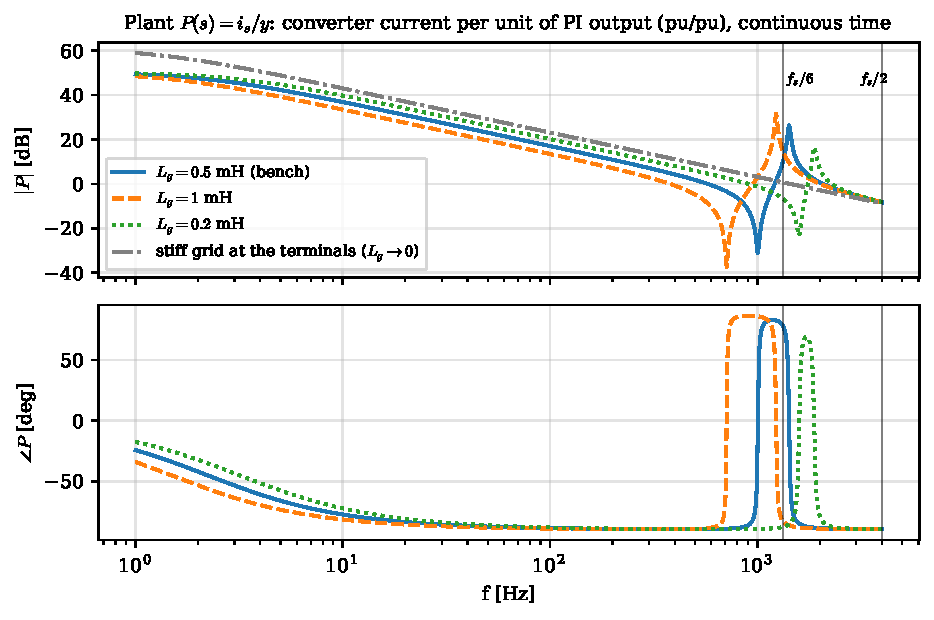
\includegraphics[width=0.9\linewidth]{figures/fig_plant_bode.pdf}
\caption{Plant $P(s) = i_s/y$ (converter current per unit of controller output, continuous time) for three values of the line inductance and for a stiff grid at the terminals. The LCL resonance moves from \SI{1.4}{kHz} (bench) to \SI{1.2}{kHz} with \SI{1}{mH} of line and to \SI{1.9}{kHz} with \SI{0.2}{mH}; $f_s/6$ and $f_s/2$ are marked.}
\label{fig:plant}
\end{figure}

\subsection{Three-level modulation}
\label{sec:modulation}

Each T-type leg produces three voltages against the neutral point, $+u_{dc}/2$ ($Q_1$ on), $0$ ($Q_2$ and $Q_3$ on) and $-u_{dc}/2$ ($Q_4$ on). With the reference $m \in [-1, 1]$ of leg $u$ compared with the carrier $r \in [0, 1]$ (Sect.~\ref{sec:modulator}), in the positive half-wave the leg switches between $+u_{dc}/2$ and $0$ with duty $m$ and in the negative one between $0$ and $-u_{dc}/2$ with duty $-m$; leg $v$ does the same with $-m$. The bridge voltage $u_s = u_u - u_v$ therefore takes the values $0$, $\pm u_{dc}/2$ and $\pm u_{dc}$ and, with the two legs on the same carrier, its first switching harmonic is at $2f_{pwm}$ (Fig.~\ref{fig:modulator}); its average over a switching period is $m\,u_{dc}$. The current ripple is that of a two-level bridge at twice the frequency and half the voltage,
\begin{equation}
\Delta i_{pp,max} = \frac{u_{dc}/2}{4\,L_c}\,\frac{1}{2f_{pwm}} = \SI{25}{A} \quad (\SI{14}{\percent}\text{ of } i_{bez}),
\label{eq:ripple}
\end{equation}
at the worst duty. The dead time between $Q_1$ and $Q_3$ ($Q_4$ and $Q_2$) is \SI{300}{ns}, quantized to the block step $\tc$.

% =====================================================================================================
\section{Control structure}
\label{sec:structure}

\subsection{Overview}
\label{sec:overview}

Fig.~\ref{fig:ctrl} is the block diagram of the control as coded in \code{afe\_sp\_ttype\_ctrl\_pwm} (signal names as in the code and in the log index \code{afe\_single\_phase\_ttype\_log\_index.m}). The chain, executed once per control step, is:
\begin{enumerate}
\item \textbf{Acquisitions.} $i_s$, $u_{ac}$, $u_{dc}$ (and the two bank voltages) sampled at the TRGO, quantized, used at the next step; an optional Gaussian noise ($\sigma = 0.01\pu$ by default, the band-limited white noise of the bench model) is added to the current sample.
\item \textbf{Clock alignment.} A PI on the difference between the master time and the local clock corrects the local clock from the next step; with zero gains (the default) the local clock is the master time. It keeps the carriers of several blocks aligned and does not interact with the loops.
\item \textbf{Single-phase PLL.} The terminal voltage $u_g = u_{ac}/u_{g,nom}$ is the $\alpha$ component of a virtual vector whose $\beta$ component is generated by a first-order low pass in the synchronous frame fed back to the stationary one (Sect.~\ref{sec:pllstructure}); the PI on the quadrature component $u_\eta$ drives the angle $\theta$, and a double-integrator observer on $\theta$ gives $\hat\theta$, the angle of every frame transformation of the control, and the frequency estimate $\hat\omega$.
\item \textbf{First harmonic tracker (FHT).} A resonant observer on the acquired current gives the fundamental $\ihat_\alpha$ and its quadrature $\ihat_\beta$ (Sect.~\ref{sec:fhtstructure}); the pair is rotated into the dq frame of $\hat\theta$: $i_d$, $i_q$.
\item \textbf{References.} Mode 0: $i_d^*$ is a rate-limited step (\SI{1}{pu} from \SI{0.35}{s} with \SI{2}{pu/s} by default), $i_q^* = i_{q,ref}$. Mode 1: $i_d^*$ is the output of the DC-link voltage loop (Sect.~\ref{sec:dclinkstructure}), negative when the DC link must charge. Positive $i_d$ is current out of the bridge in phase with the terminal voltage: power from the DC link to the AC side.
\item \textbf{Current loop.} Vector PI ($\kpi$, $\kii$) on $(i_d^* - i_d,\ i_q^* - i_q)$; the outputs are divided by the acquired DC-link voltage (feed-forward) and limited to the unit circle, giving the modulation vector $(m_d, m_q)$ with a clip flag for the next step. At the first step after the enable the integrators are pre-loaded with the terminal voltage (bumpless start).
\item \textbf{Modulation.} $m = m_d\cos\hat\theta - m_q\sin\hat\theta$, the $\alpha$ component of the modulation vector, is the reference of leg $u$; leg $v$ gets $-m$; the gate commands with the dead time are computed every $\tc$ (Sect.~\ref{sec:modulator}).
\end{enumerate}
The gates are off and the loops at rest until the first control step with $t \ge t_{enable}$ (\SI{0.1}{s}, about three grid periods for the PLL to lock). In the master/slave mode (modules in series on one line) the slave runs its acquisitions, its PLL and its FHT, skips the loops and applies $(m_d, m_q)$ of the master rotated with its own PLL angle, so that identical modules in series produce the same voltage; the master runs before the slave in the same $\tc$ step, so the slave uses the command of the same trigger.

\begin{figure}[htb]
\centering
\resizebox{\linewidth}{!}{%
\begin{tikzpicture}[>=Latex, font=\footnotesize,
  blk/.style={draw, minimum height=7mm, minimum width=11mm, inner sep=3pt, align=center, fill=gray!8},
  sum/.style={draw, circle, minimum size=4mm, inner sep=0pt},
  lbl/.style={inner sep=1.5pt}]
% PLL row
\node[blk, minimum width=18mm] (acq) at (0,0) {acquisitions \\ $z^{-1}$, quantizer};
\node[lbl, left=4mm of acq, align=right] (meas) {$i_s$, $u_{ac}$, $u_{dc}$};
\draw[->] (meas) -- (acq);
\node[blk, minimum width=24mm] (pll) at (3.6,1.6) {single-phase PLL \\ virtual $\beta$, PI, observer};
\draw[->] (acq.east) ++(0,0.15) -- ++(0.4,0) |- node[right, lbl, pos=0.3] {$u_{ac}/u_{g,nom}$} (pll.west);
% FHT row
\node[blk, minimum width=24mm] (fht) at (3.6,0) {FHT \\ $\ihat_\alpha$, $\ihat_\beta$};
\draw[->] (acq.east) -- node[above, lbl] {$i_s$} (fht.west);
\node[blk] (rot1) at (6.6,0) {$\ee^{-\jj\hat\theta}$};
\draw[->] (fht) -- (rot1);
\draw[->] (pll.east) -| node[right, lbl, pos=0.85] {$\hat\theta$} (rot1.north);
% current loop
\node[sum] (s1) at (8.3,0) {};
\draw[->] (rot1) -- node[above, lbl] {$i_d$, $i_q$} (s1);
\node[lbl, below right=-0.5mm and -0.5mm of s1] {$-$};
\node[blk, minimum width=20mm] (pi) at (10.4,0) {vector PI \\ $\kpi + \kii/s$};
\draw[->] (s1) -- (pi);
\node[blk] (ff) at (12.9,0) {$\div\,u_{dc}$};
\draw[->] (pi) -- node[above, lbl] {$y_d$, $y_q$} (ff);
\node[blk] (lim) at (14.7,0) {$|\vec m| \le 1$};
\draw[->] (ff) -- (lim);
\draw[->] (acq.east) ++(0,-0.15) -- ++(0.3,0) |- (3.0,-2.3) -- (12.9,-2.3) -- (ff.south);
\node[lbl, above] at (8.0,-2.3) {$u_{dc}$ (saturated at $u_{dc,min}$)};
% references
\node[blk, minimum width=24mm] (ref) at (8.3,1.6) {references \\ mode 0: ramp; mode 1: $u_{dc}$ loop};
\draw[->] (ref.south) -- node[right, lbl] {$i_d^*$, $i_q^*$} (s1.north);
% modulation
\node[blk] (rot2) at (14.7,-1.3) {$\Re[\,\cdot\,\ee^{\jj\hat\theta}]$};
\draw[->] (lim.south) -- node[right, lbl] {$m_d$, $m_q$} (rot2.north);
\node[blk, minimum width=22mm] (pwm) at (11.2,-1.3) {three-level PWM \\ leg $u$: $m$, leg $v$: $-m$};
\draw[->] (rot2) -- node[above, lbl] {$m$} (pwm);
\node[lbl, left=4mm of pwm] (gates) {$G$ (8 gates)};
\draw[->] (pwm) -- (gates);
% sync
\node[lbl, align=center] (sync) at (14.7,1.5) {\code{sync} to the slave \\ $\hat\theta$, $m_d$, $m_q$};
\draw[->, dashed] (lim.north) -- (sync);
\end{tikzpicture}}
\caption{Control of one module as coded in \code{afe\_sp\_ttype\_ctrl\_pwm}. The current loop acts on the fundamental of the single-phase current, estimated with its quadrature by the FHT and rotated into the dq frame of the PLL angle $\hat\theta$; the modulation index is the $\alpha$ component of the modulation vector. A slave applies $(m_d, m_q)$ of the master with its own $\hat\theta$.}
\label{fig:ctrl}
\end{figure}

\subsection{Single-phase PLL}
\label{sec:pllstructure}

A single-phase voltage has no quadrature component to measure. The PLL builds a virtual vector $\vec u = u_g + \jj u_\beta$ from the acquired $u_g = u_{ac}/u_{g,nom}$ (per unit of the nominal grid amplitude, so that $|\vec u| \simeq 1$) and from a $\beta$ component generated by the PLL itself: the vector is rotated into the PLL frame, $u_\xi + \jj u_\eta = \vec u\,\ee^{-\jj\theta}$, both components are passed through a first-order low pass of time constant $\tau = 2/\wo = \SI{6.4}{ms}$, and the $\beta$ component of the filtered vector rotated back to the stationary frame is the $u_\beta$ of the next step:
\begin{equation}
u_\beta = \Im\!\left[\left(\frac{1}{1 + \tau s}\,\vec u\,\ee^{-\jj\theta}\right)\ee^{\jj\theta}\right].
\label{eq:virtual_beta}
\end{equation}
The in-phase component is \emph{not} filtered: $u_\xi$, $u_\eta$ are formed from the raw $u_g$ and the virtual $u_\beta$. Sect.~\ref{sec:sogi} shows that (\ref{eq:virtual_beta}) with a locked PLL is exactly the quadrature output of a second-order generalized integrator (SOGI-QSG \cite{ciobotaru2006}) with $k = 1/(\tau\wo) = 0.5$: $u_\beta$ is the fundamental of $u_g$ delayed by \SI{90}{\degree}, with unit gain at $\wo$ and the harmonics attenuated. The PI on $u_\eta$ ($k_{p,pll} = 1$, $k_{i,pll} = 0$: a type-1 loop, Sect.~\ref{sec:pllloop}), with the output limited to $\pm 2$ and back-calculation anti-windup, gives the frequency correction in per unit of $\omega_{nom}$: $\theta(k+1) = \theta(k) + \omega_{nom}\ts\,(1 + y_{pll})$, wrapped to $[-\pi, \pi)$. Finally a double-integrator observer with the poles at $\ee^{-\wo\ts}$, $\ee^{-4\wo\ts}$ (gains $l_1 = 0.184$, $l_2 = \SI{44.8}{s^{-1}}$) follows $\theta$ and provides the angle $\hat\theta$ used by every frame transformation and the frequency estimate $\hat\omega$; it smooths the angle (the PLL angle carries the ripple of $u_\eta$) and makes the frequency available for the log and for the bumpless start.

\subsection{First harmonic tracker on the current}
\label{sec:fhtstructure}

The converter current has one physical component. Its fundamental and the quadrature of the fundamental are estimated by a Luenberger observer whose internal model is the oscillator at $\wo$ (the harmonic observer of the first issue of this note),
\begin{equation}
\dot x_1 = x_2, \qquad \dot x_2 = -\wo^2 x_1 - \delta\wo x_2, \qquad
\dot{\hat x} = A\hat x + L\,(i_s - \hat x_1), \quad L = [l_1\ \ l_2]^T,
\label{eq:fht_model}
\end{equation}
with the poles of $A - LC$ placed at $-\wo$ and $-4\wo$ and the small damping $\delta = 0.05$ in the internal model (as in the Simulink block of the bench). The outputs are the in-phase estimate $\ihat_\alpha = \hat x_1$ and the quadrature estimate $\ihat_\beta = -\hat x_2/\wo$: for $\hat x_1 = I\cos(\wo t + \varphi)$ the second state is $\hat x_2 = -\wo I\sin(\wo t + \varphi)$, so that $\ihat_\beta = I\sin(\wo t + \varphi)$ \emph{lags} $\ihat_\alpha$ by \SI{90}{\degree}, the $\beta$ component of a vector turning at $+\wo$. The pair is rotated into the dq frame of the PLL,
\begin{equation}
i_d = \ihat_\alpha\cos\hat\theta + \ihat_\beta\sin\hat\theta, \qquad i_q = -\ihat_\alpha\sin\hat\theta + \ihat_\beta\cos\hat\theta,
\label{eq:dq}
\end{equation}
where a current at $\wo$ is a DC pair ($i_d$ in phase with the terminal voltage, $i_q$ in quadrature). The transfer functions of the two outputs from the acquired current are
\begin{equation}
\Hu(s) = \frac{\ihat_\alpha}{i_s} = \frac{l_1 s + l_1\delta\wo + l_2}{\Delta(s)}, \qquad
\Hv(s) = \frac{\ihat_\beta}{i_s} = -\frac{l_2 s - l_1\wo^2}{\wo\,\Delta(s)},
\label{eq:fht_tf}
\end{equation}
with the characteristic polynomial of the observer $\Delta(s) = s^2 + (l_1 + \delta\wo)s + \wo^2 + l_2 + l_1\delta\wo$ and, for the poles at $-a\wo$ and $-b\wo$ ($a = 1$, $b = 4$), $l_1 = (a + b - \delta)\wo = \SI{1555}{s^{-1}}$ and $l_2 = (ab - 1 - (a + b - \delta)\delta)\wo^2 = 2.72\cdot10^{5}\,\mathrm{s^{-2}}$ (the discrete gains of the code, $l_1 = 0.182$ and $l_2 = \SI{29.6}{s^{-1}}$ per step, are $L\ts$ within a few percent, Sect.~\ref{sec:disc_fht}). With $\delta = 0$, $\Delta(\jj\wo) = l_2 + \jj l_1\wo$ and $\Hu(\jj\wo) = 1$, $\Hv(\jj\wo) = -\jj$ for \emph{any} observer gains: the estimate reproduces the component at $\wo$ exactly and the quadrature output lags it by exactly \SI{90}{\degree}; the gains set the dynamics (slow time constant $1/\wo = \SI{3.2}{ms}$, settling of the estimates within \SI{2}{\percent} in about \SI{13}{ms}) and the selectivity. With $\delta = 0.05$ the tracking is approximate, $\Hu(\jj\wo) = 0.993\,\angle\SI{-0.25}{\degree}$ and $\Hv(\jj\wo) = 0.971\,\angle\SI{-88.1}{\degree}$ in continuous time; the discrete form as coded happens to be closer (Sect.~\ref{sec:disc_fht}). Fig.~\ref{fig:fht} shows the two responses: above the fundamental $\Hu$ falls as $l_1/(s + l_1)$, a first-order low pass with the corner at \SI{248}{Hz} ($|\Hu| = 0.17$ at the LCL resonance, $0.46$ at \SI{500}{Hz}), and this low-pass character is what the current loop sees; at DC both outputs are finite, $\Hu(0) = (ab - 1)/(ab) = 0.75$ and $\Hv(0) = (a + b - \delta)/(ab) = 1.24$, which is the origin of the DC mode of Sect.~\ref{sec:dcmode}.

\begin{figure}[htb]
\centering
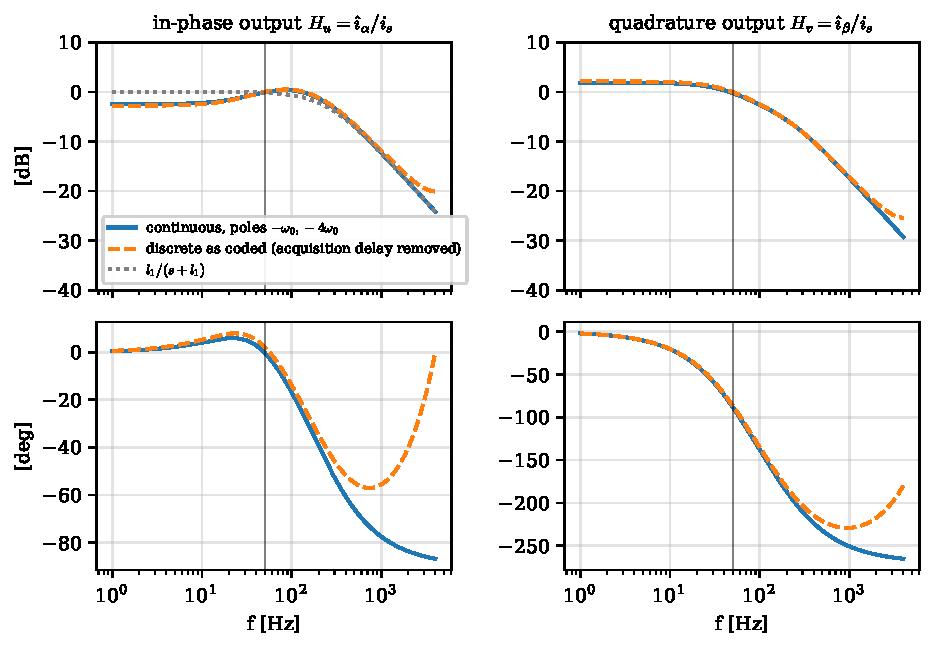
\includegraphics[width=0.95\linewidth]{figures/fig_fht.pdf}
\caption{Frequency response of the FHT from the acquired current to the in-phase estimate $\ihat_\alpha$ (left) and to the quadrature estimate $\ihat_\beta$ (right), continuous time and discrete form as coded (acquisition delay removed). Above the fundamental $\Hu$ is the low pass $l_1/(s + l_1)$ (dotted); at DC the two outputs are 0.75 and 1.24.}
\label{fig:fht}
\end{figure}

\subsection{Current loop with the DC-link feed-forward}
\label{sec:currentctrl}

The vector PI acts on the dq errors with the same real gains on the two axes,
\begin{equation}
y_d = \kpi\,(i_d^* - i_d) + \frac{\kii}{s}\,(i_d^* - i_d), \qquad y_q = \kpi\,(i_q^* - i_q) + \frac{\kii}{s}\,(i_q^* - i_q),
\label{eq:pi}
\end{equation}
without decoupling terms and without a voltage feed-forward: the grid voltage is built up by the integrators (and pre-loaded at the enable). This is the single-phase dq control of \cite{zhang2002}, with the quadrature component generated by the FHT instead of a transport delay or a SOGI. The outputs are voltages in per unit of $u_{dc,nom}$; the DC-link feed-forward divides them by the acquired DC-link voltage, saturated below at $u_{dc,min} = 0.25\pu$,
\begin{equation}
m_d = \frac{y_d}{\max(u_{dc}, u_{dc,min})}, \qquad m_q = \frac{y_q}{\max(u_{dc}, u_{dc,min})},
\label{eq:ff}
\end{equation}
so that the bridge produces the voltage the PI asks for whatever the DC-link voltage (the loop gain does not depend on $u_{dc}$ and the \SI{100}{Hz} ripple of the single-phase DC link is compensated, up to the one-step delay of the sample, Sect.~\ref{sec:disc_ff}). The vector is then limited to the unit circle, $|\vec m| \le u_{lim} = 1$, with a clip flag that at the next step stops the integrators (Sect.~\ref{sec:limits}). The modulation index of leg $u$ is the $\alpha$ component of the modulation vector, $m = \Re[(m_d + \jj m_q)\,\ee^{\jj\hat\theta}] = m_d\cos\hat\theta - m_q\sin\hat\theta$. The default gains of the library are $\kpi = 0.1$, $\kii = \SI{20}{s^{-1}}$; the bench model used $0.5$ and \SI{45}{s^{-1}} with an earlier filter. Sect.~\ref{sec:analysis} analyses the loop and recommends $\kpi = 0.15$, $\kii = \SI{20}{s^{-1}}$.

\subsection{DC-link voltage loop (mode 1)}
\label{sec:dclinkstructure}

In mode 1 the module regulates its DC-link voltage with the current it exchanges with the grid (the DC link is then fed by a source, a DC transformer or a load). The reference $u_{dc}^*$ is reached through a first-order low pass ($\tau_{ref} = \SI{20}{ms}$) from the voltage measured at the first trigger; the measurement is averaged over one grid period ($N = 160$ samples, a moving average with exact zeros at every multiple of \SI{50}{Hz}) and optionally low-passed again; the PI ($\kpu = 2$, $\kiu = \SI{20}{s^{-1}}$) with the output saturated at $\pm i_{lim} = \pm 1.2\pu$ and back-calculation anti-windup gives the current reference $i_d^* = -y_{udc}$, a current \emph{into} the bridge when the DC link must charge. The moving average removes from the loop the \SI{100}{Hz} ripple of the single-phase DC link (\SI{66}{V} peak-peak at full load with \SI{3}{mF}) and the \SI{50}{Hz} ripple that a DC offset of the current produces on the DC-link voltage, at the cost of \SI{10}{ms} of delay in the loop (Sect.~\ref{sec:dclink}).

\subsection{Limiters, anti-windup, enable and master/slave}
\label{sec:limits}

The current PI ends in the circular limiter of radius $u_{lim} = 1$ applied \emph{after} the division by $u_{dc}$, and raises the clip flag when $|\vec m| \ge u_{lim}$; the flag is used at the next step: while it is set the integrator inputs are removed and the states are held with a leak, $x \leftarrow (1 - c_{rel}\ts)\,x$ with $c_{rel} = \SI{0.001}{s^{-1}}$, numerically a hold, and the proportional part keeps acting on the error. The PLL PI and the DC-link PI use the back-calculation form (the integrator state is set to the saturated output minus the proportional part). The current reference of mode 0 is rate limited (\SI{2}{pu/s}) and that of mode 1 saturated at $\pm i_{lim}$. The modulation index is saturated in $[m_{low}, m_{up}] = [-1, 1]$ by the modulator.

Before the enable the gates are off, the PI integrators and the current reference are zero and the PLL runs; at the first enabled control step the integrators are pre-loaded with the terminal voltage, rotated by $1.5\,\hat\omega\ts$ to account for the acquisition delay and the hold,
\begin{equation}
(x_d, x_q) = \frac{u_{g,nom}\,u_{bez}}{u_{dc,nom}}\,(u_\xi + \jj u_\eta)\,\ee^{\jj 1.5\hat\omega\ts},
\label{eq:bumpless}
\end{equation}
so that the bridge starts at the grid voltage and the current starts from zero without inrush (\SI{0.000}{pu} of peak in the simulation of Sect.~\ref{sec:verification}); the gates follow the enable state of the last control step, so the bridge starts switching at that step with the pre-loaded index and never between two triggers with a stale one. The clip handling and the limiters are the only nonlinearities of the controller: the analysis of the next sections is linear and holds while no limiter is active.

% =====================================================================================================
\section{Analysis of the current loop}
\label{sec:analysis}

\subsection{The exact stationary-frame equivalent}
\label{sec:equivalence}

The loop of Fig.~\ref{fig:ctrl} looks time-varying: a rotation by $-\hat\theta$, a PI, a rotation by $+\hat\theta$ and a projection on one axis. With the PLL locked, $\hat\theta = \wo t$ (a constant offset is immaterial), it is in fact linear time-invariant and can be written exactly as a single-input single-output controller in the stationary frame. Let $\tilde\imath = \ihat_\alpha + \jj\ihat_\beta = [\Hu(s) + \jj\Hv(s)]\,i_s$ be the complex estimate of the FHT, a complex-coefficient filter acting on the real current, and $C(s) = \kpi + \kii/s$ the PI acting with the same real gains on the complex error. With zero references the output of the PI is $y_d + \jj y_q = -C(s)\,[\tilde\imath\,\ee^{-\jj\wo t}]$, and the frequency-shift property of a linear filter, $\ee^{\jj\wo t}\,C(s)[x\,\ee^{-\jj\wo t}] = C(s - \jj\wo)[x]$, gives for the rotated output
\begin{equation}
(y_d + \jj y_q)\,\ee^{\jj\wo t} = -C(s - \jj\wo)\,[\Hu(s) + \jj\Hv(s)]\,i_s .
\label{eq:shift}
\end{equation}
The modulation index is the real part of this vector, and the real part of a complex-coefficient filter $G(s)$ acting on a real signal is the real filter $\tfrac12[G(s) + G^*(s)]$, $G^*$ having the conjugate coefficients. The controller seen by the plant is therefore
\begin{equation}
\Ceq(s) = \tfrac12\left[C(s - \jj\wo)\,(\Hu + \jj\Hv) + C(s + \jj\wo)\,(\Hu - \jj\Hv)\right]
= \kpi\,\Hu(s) + \kii\,\frac{s\,\Hu(s) - \wo\,\Hv(s)}{s^2 + \wo^2},
\label{eq:ceq}
\end{equation}
a proportional-resonant controller \cite{zmood2003, teodorescu2006} shaped by the two outputs of the FHT: the proportional path passes through the in-phase output, the resonant path uses both. Three limiting cases make the structure clear. Without the quadrature estimate ($\Hu = 1$, $\Hv = 0$) the controller is the plain PR $\kpi + \kii s/(s^2 + \wo^2)$. With an \emph{ideal} tracker ($\Hu = 1$, $\Hv(\jj\omega) = -\jj$ for $\omega > 0$) it is the single-sided complex PI $\kpi + \kii/(s - \jj\wo)$, the exact image of the synchronous PI on a vector turning at $+\wo$ \cite{zmood2001}, whose residue at $\jj\wo$ is $\kii$, the same as that of the PR $\kpi + 2\kii s/(s^2 + \wo^2)$; this is the reference curve of Fig.~\ref{fig:ceq}. With the real FHT the residue at $\jj\wo$ is $\kii\,[\jj\wo\Hu(\jj\wo) - \wo\Hv(\jj\wo)]/(2\jj\wo)$, equal to $\kii$ when the tracking is exact at $\wo$ ($\Hu = 1$, $\Hv = -\jj$): the infinite gain at the fundamental, hence the zero steady-state error on $i_d$ and $i_q$, does not depend on the FHT gains, only on the exactness of its internal model at $\wo$ (Sect.~\ref{sec:disc_fht}). Away from the fundamental the FHT shapes the controller: above \SI{248}{Hz} both outputs fall as $1/s$ and the proportional path becomes the low pass $\kpi l_1/(s + l_1)$; at DC the controller has the finite gain
\begin{equation}
\Ceq(0) = \kpi\Hu(0) - \frac{\kii}{\wo}\,\Hv(0) = \frac{ab - 1}{ab}\,\kpi - \frac{a + b - \delta}{ab}\,\frac{\kii}{\wo} = 0.75\,\kpi - 1.24\,\frac{\kii}{\wo},
\label{eq:ceq0}
\end{equation}
which is \emph{negative} when $\kii/\kpi > \wo(ab - 1)/(a + b - \delta) = \SI{190}{rad/s}$ (Sect.~\ref{sec:dcmode}).

The same derivation holds in discrete time with the PI as coded, $C(z) = \kpi + \kii\ts\,z/(z - 1)$, and the shift $z \to z\,\ee^{\mp\jj\wo\ts}$:
\begin{equation}
\Ceq(z) = \kpi\,\Hu(z) + \kii\ts\,\frac{z\,[(z - \cos\wo\ts)\,\Hu(z) - \sin(\wo\ts)\,\Hv(z)]}{z^2 - 2\cos(\wo\ts)\,z + 1},
\label{eq:ceq_z}
\end{equation}
where $\Hu(z)$, $\Hv(z)$ are the responses of the discrete FHT from the acquired sample to the estimates used in the step (Sect.~\ref{sec:disc_fht}). The resonant denominator has its roots exactly at $\ee^{\pm\jj\wo\ts}$: the frame rotations are exact operations and the PI integrator has its pole at $z = 1$ with any discretization, so the discrete controller has infinite gain at exactly $\wo$ without any care in the discretization of the PI. The rest of the loop is the one-step acquisition delay and the plant with the zero-order hold,
\begin{equation}
L(z) = \Ceq(z)\,z^{-1}\,\kmod\,P_{zoh}(z), \qquad P_{zoh}(z) = \mathcal{Z}\!\left\{\frac{1 - \ee^{-s\ts}}{s}\,\frac{P(s)}{\kmod}\right\},
\label{eq:loop}
\end{equation}
and the closed-loop poles are the roots of $z\,d_C(z)\,d_P(z) + n_C(z)\,n_P(z)$ with $\Ceq = n_C/d_C$ and $\kmod P_{zoh} = n_P/d_P$. The equivalence is exact as long as the PLL is locked and no limiter is active; the simulation of Sect.~\ref{sec:verification}, which runs the controller as coded with its PLL, confirms every pole it predicts.

\begin{figure}[htb]
\centering
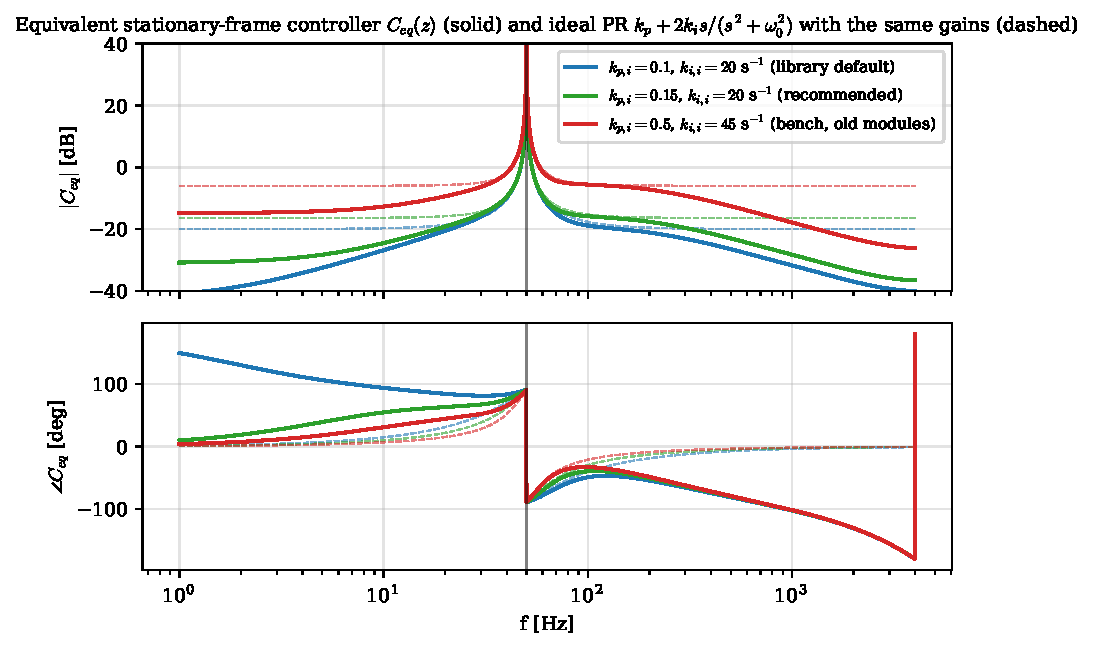
\includegraphics[width=0.95\linewidth]{figures/fig_ceq.pdf}
\caption{Equivalent stationary-frame controller $\Ceq(z)$ for the three gain sets (solid) and the ideal PR $\kpi + 2\kii s/(s^2 + \wo^2)$ with the same gains (dashed, the same residue at the fundamental). The FHT turns the proportional gain into a low pass above \SI{248}{Hz} and gives the controller a finite DC gain, negative for the library default (phase \SI{180}{\degree} below \SI{20}{Hz}).}
\label{fig:ceq}
\end{figure}

\subsection{Loop gain, crossover and margins}
\label{sec:margins}

Below the resonance the plant is the integrator (\ref{eq:plant_lf}) and the proportional path of the controller is $\kpi\Hu$: the crossover is, to first order,
\begin{equation}
\omega_c \simeq \kpi\,\frac{\kmod}{L_c' + L_g'}\,|\Hu(\jj\omega_c)|, \qquad \kpi\,\frac{\kmod}{L_c' + L_g'} = \SI{676}{rad/s} \ \text{for } \kpi = 0.15,
\label{eq:wc}
\end{equation}
\SI{705}{rad/s} (\SI{112}{Hz}) from the exact loop (\ref{eq:loop}), where $|\Hu| = 1.04$ and the resonant path still adds \SI{45}{\percent} of the proportional one in quadrature ($|\Ceq(\jj\omega_c)| = 0.157$, phase \SI{-39.2}{\degree}). The phase margin is the sum of three contributions: the plant with the hold, \SI{-91.4}{\degree}; the acquisition delay, \SI{-5.0}{\degree}; and the controller, \SI{-39.2}{\degree}, of which about \SI{-22}{\degree} are the lag of the in-phase output of the FHT at the crossover ($\Hu(\jj\omega_c) = 1.04\,\angle\SI{-22.3}{\degree}$, one step included) and the rest the phase of the resonant path: $\varphi_m = \SI{44.4}{\degree}$ for the recommended gains. Table~\ref{tab:gains} collects the figures of the three gain sets of interest and of a few candidates, Fig.~\ref{fig:loop} the open-loop responses and Fig.~\ref{fig:nyquist} the Nyquist plots. The FHT costs about \SI{15}{\degree} of phase margin against an ideal PR with the same gains ($\varphi_m = \SI{59.3}{\degree}$, \SI{117}{Hz}); what it buys is described in the next section.

\begin{table}[htb]
\centering\footnotesize\setlength{\tabcolsep}{4pt}
\caption{Current loop with $L_g = \SI{0.5}{mH}$ and the resistance of the model: crossover, phase margin, loop gain at the LCL resonance, modulus margin $\min|1 + L|$, real closed-loop pole of the DC mode, damping rate of the closed-loop pair near the fundamental and line inductance above which the LCL mode becomes unstable. Boldface: library default (0.1/20), recommended (0.15/20) and old bench gains (0.5/45, unstable already at \SI{0.5}{mH}: LCL mode $\sigma = \SI{+57}{s^{-1}}$).}
\label{tab:gains}
\begin{tabular}{@{}llccccccc@{}}
\toprule
$\kpi$ & $\kii$ [s$^{-1}$] & $f_c$ [Hz] & $\varphi_m$ [deg] & $|L(\jj\wres)|$ & $\min|1+L|$ & DC pole [s$^{-1}$] & LF pair $\sigma$ [s$^{-1}$] & $L_g$ limit [mH] \\
\midrule
\textbf{0.1} & \textbf{20} & 88 & 32.5 & 0.37 & 0.56 & $\mathbf{+5.1}$ (unstable) & $-90$ & 1.45 \\
0.1 & 15 & 84 & 39.3 & 0.37 & 0.66 & $-18.8$ & $-79$ & 1.45 \\
0.12 & 15 & 93 & 46.1 & 0.45 & 0.60 & $-34.7$ & $-86$ & 1.15 \\
0.12 & 20 & 96 & 39.7 & 0.45 & 0.60 & $-9.9$ & $-106$ & 1.15 \\
\textbf{0.15} & \textbf{20} & 112 & 44.4 & 0.56 & 0.50 & $-30.0$ & $-109$ & 0.90 \\
0.15 & 15 & 111 & 48.8 & 0.56 & 0.50 & $-55.2$ & $-84$ & 0.90 \\
0.15 & 30 & 115 & 36.4 & 0.56 & 0.50 & $+6.7$ (unstable) & $-154$ & 0.90 \\
0.2 & 20 & 141 & 42.4 & 0.74 & 0.36 & $-57.5$ & $-94$ & 0.70 \\
\textbf{0.5} & \textbf{45} & 263 & 15.0 & \textbf{1.86} & 0.22 & $-72.5$ & $-95$ & 0.40 \\
\bottomrule
\end{tabular}
\end{table}

\begin{figure}[htb]
\centering
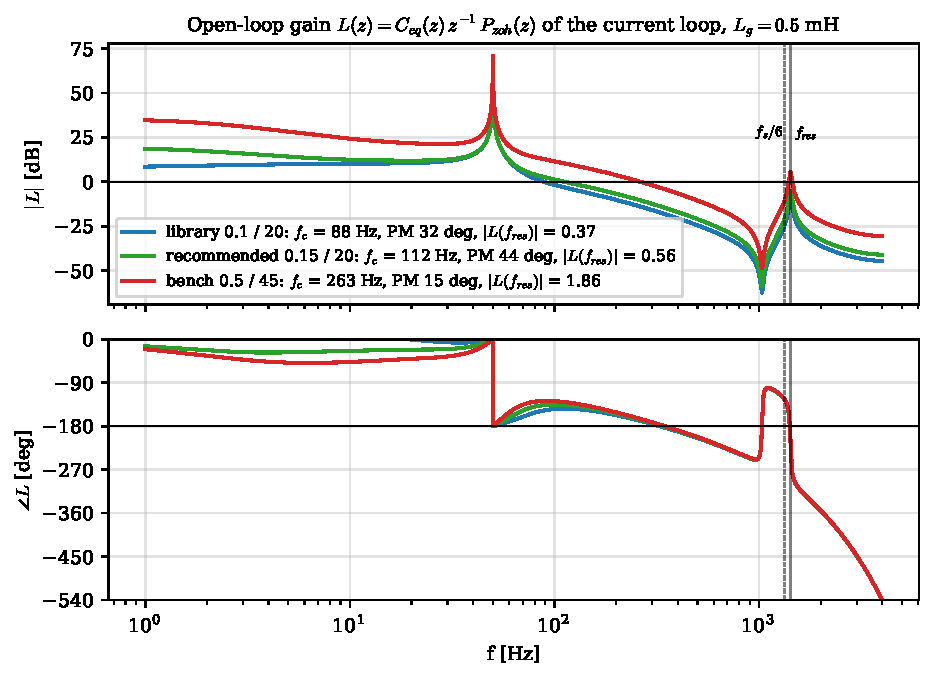
\includegraphics[width=0.95\linewidth]{figures/fig_loop_bode.pdf}
\caption{Open-loop gain of the current loop (\ref{eq:loop}) for the three gain sets, $L_g = \SI{0.5}{mH}$. The phase is beyond \SI{-180}{\degree} at the LCL resonance (above $f_s/6$): the resonance is stable only if the gain there is below one, which holds for the library and the recommended gains and fails for the old bench gains.}
\label{fig:loop}
\end{figure}

\begin{figure}[htb]
\centering
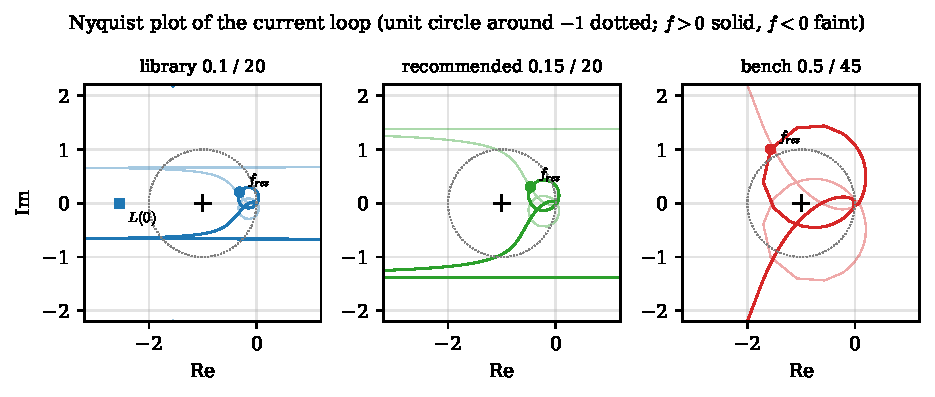
\includegraphics[width=0.95\linewidth]{figures/fig_nyquist.pdf}
\caption{Nyquist plots of the three gain sets. Library default: the plot starts at $L(0) = -2.55$, to the left of $-1$, and the DC mode is unstable; recommended: $L(0) = +9.2$, the loop around the resonance stays inside the unit circle; old bench gains: the resonance loop encircles $-1$.}
\label{fig:nyquist}
\end{figure}

\subsection{The LCL resonance above $f_s/6$: gain stabilization by the FHT}
\label{sec:resonance}

At the LCL resonance the phase of the delayed plant is below \SI{-180}{\degree} (Fig.~\ref{fig:loop}): with the resonance above $f_s/6$ the converter-current feedback adds negative damping to it \cite{parker2014}, and the only way to keep it stable without an additional damping loop is to keep the loop gain there below one. The plant gain at the resonance is large, limited by $R_{cf}$ only (a factor 20, \SI{26}{dB}, for $\kmod P_{zoh}$ at \SI{1424}{Hz}), and an ideal PR with the recommended gains would give $|L(\jj\wres)| = 3.16$: unstable. The in-phase output of the FHT, $|\Hu| = 0.185$ at the resonance (discrete form as coded), brings it to $0.56$: the FHT is the low-pass filter that gain-stabilizes the resonance, at the cost of the phase margin of the previous section. The rule for the gains is then
\begin{equation}
|L(\jj\wres)| \simeq \kpi\,|\Hu(\jj\wres)|\,\kmod\,|P_{zoh}(\ee^{\jj\wres\ts})| < 1 \quad\Longrightarrow\quad \kpi < 0.27 \ \text{for } L_g = \SI{0.5}{mH},
\label{eq:gain_stab}
\end{equation}
and the old bench gains ($\kpi = 0.5$, tuned on the earlier filter) violate it: $|L(\jj\wres)| = 1.86$, closed-loop LCL mode at $\sigma = \SI{+57}{s^{-1}}$, the current grows to the limiter within a few tens of milliseconds (Fig.~\ref{fig:gains}). The margin left by $\kpi = 0.15$ is modest ($0.56$, closed-loop LCL mode at $\sigma = \SI{-55}{s^{-1}}$ against $-107$ in open loop: the loop halves the natural damping of the resonance) and it depends on the line inductance: Fig.~\ref{fig:robust} shows the margins as a function of $L_g$. A weaker grid lowers the resonance and raises the plant gain there; the LCL mode of the recommended gains becomes unstable for $L_g > \SI{0.91}{mH}$ ($\fres = \SI{1253}{Hz}$), that of the library gains for $L_g > \SI{1.45}{mH}$ (while their DC mode is unstable for any $L_g$). Towards a stiff grid the resonance moves up and out of the way ($L_g = \SI{0.05}{mH}$: \SI{3.3}{kHz}, $|L| = 0.01$) and the crossover rises to \SI{180}{Hz} with \SI{31}{\degree} of margin, the FHT lag growing with the crossover. Where a weaker grid is expected, the line inductor should be included in $L_g$ when the resonance is checked, or the gain reduced, or an active damping added (not implemented); the bench, with \SI{0.5}{mH} of line inductor per module and the leakage of the grid transformer, sits at $\fres \simeq \SI{1.4}{kHz}$.

\begin{figure}[htb]
\centering
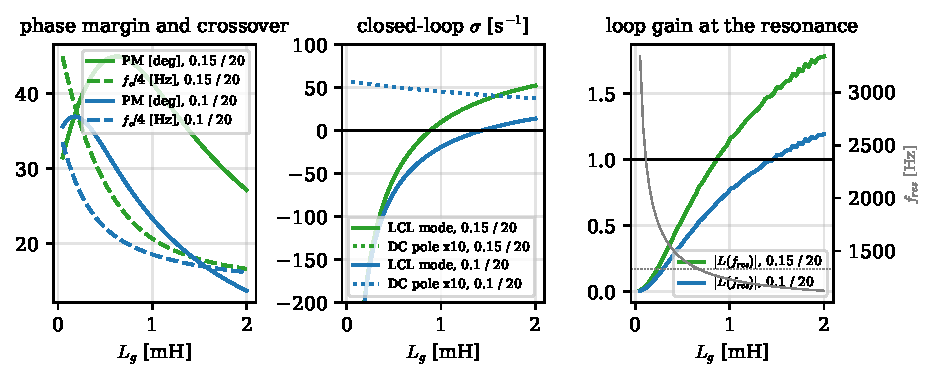
\includegraphics[width=0.98\linewidth]{figures/fig_robust_lg.pdf}
\caption{Margins of the current loop as a function of the line inductance for the recommended (solid) and the library (dashed) gains: phase margin and crossover (left), damping rate of the closed-loop LCL mode and DC pole (centre), loop gain at the resonance with the resonance frequency (right). The LCL mode of the recommended gains is stable up to \SI{0.91}{mH}; the DC pole of the library gains is positive for any $L_g$.}
\label{fig:robust}
\end{figure}

\subsection{The DC mode}
\label{sec:dcmode}

A DC component of the converter current is not a fundamental, but the FHT has no state to attribute it to: it leaks into both outputs with the gains $\Hu(0) = 0.75$ and $\Hv(0) = 1.24$ of (\ref{eq:ceq0}), i.e. a DC current $I_0$ appears in the dq frame as a vector of amplitude $\sqrt{0.75^2 + 1.24^2}\,I_0 = 1.45\,I_0$ turning at $-\wo$ (a \SI{50}{Hz} ripple on $i_d$ and $i_q$). The PI reacts to it and the projection on $\alpha$ turns the reaction back into a DC component of the modulation index. The proportional part gives $-\kpi\Hu(0)I_0$, a negative feedback; the integral part acts on a vector turning at $-\wo$ with the gain $\kii/(-\jj\wo)$, a lead of \SI{90}{\degree} that maps the quadrature leakage $\Hv(0)I_0$ onto the $\alpha$ axis with the sign reversed: $+\kii\Hv(0)I_0/\wo$, a \emph{positive} feedback. The net DC gain of the controller is $\Ceq(0)$ of (\ref{eq:ceq0}) and the DC loop gain, with the plant (\ref{eq:plant_lf}) at $s = 0$,
\begin{equation}
L(0) = \Ceq(0)\,\frac{\kmod}{R'} = \left(0.75\,\kpi - 1.24\,\frac{\kii}{\wo}\right)\frac{\kmod}{R'}, \qquad \frac{\kmod}{R'} = 324 .
\label{eq:L0}
\end{equation}
The DC mode is stable only if $L(0) > -1$, practically if $\Ceq(0) > 0$ since $R'/\kmod$ is three per mil:
\begin{equation}
\frac{\kii}{\kpi} < \frac{ab - 1}{a + b - \delta}\,\wo = \SI{190}{rad/s}, \qquad\text{i.e.}\qquad \kpi > 1.65\,\frac{\kii}{\wo} = 0.105 \ \text{for } \kii = \SI{20}{s^{-1}}
\label{eq:dc_condition}
\end{equation}
(continuous time; the discrete form as coded gives $0.7245\kpi - 1.2761\kii/\wo$ and the limit $\kpi = 0.1066$ with the resistance of the model). The library default $\kpi = 0.1$, $\kii = \SI{20}{s^{-1}}$ has $\kii/\kpi = \SI{200}{rad/s}$: $\Ceq(0) = -0.0079$, $L(0) = -2.55$ and a closed-loop real pole at $\sigma = \SI{+5.1}{s^{-1}}$. The mode is slow (a time constant of \SI{200}{ms}) and marginal, and its sign depends on the resistance of the loop: with the on-state resistance of the devices added to the copper of the model (about \SI{18}{m\ohm} for two T-type legs, $R' = \SI{32}{m\ohm}$) the limit moves to $\kpi = 0.101$ and the pole to \SI{+0.8}{s^{-1}}; still unstable, with a time constant of about one second. In the time domain (Sect.~\ref{sec:verification}) a DC disturbance of \SI{0.01}{pu} on the bridge voltage drives the DC current up until the limiter of the modulation vector stops it at \SI{2.4}{pu} (Fig.~\ref{fig:dcoffset}); without disturbance the current of the module shows only the slow drift seeded by the noise and the quantization. Fig.~\ref{fig:stability} maps the stable region in the $(\kpi, \kii)$ plane: the DC condition (\ref{eq:dc_condition}) is the lower boundary, the gain stabilization of the resonance (\ref{eq:gain_stab}) the right one; the library default sits on the lower boundary, the old bench gains beyond the right one.

The recommended gains, $\kpi = 0.15$ and $\kii = \SI{20}{s^{-1}}$ ($\kii/\kpi = \SI{133}{rad/s}$), give $\Ceq(0) = +0.028$, $L(0) = +9.2$ and the DC pole at $\sigma = \SI{-30}{s^{-1}}$ (the open-loop pole is at \SI{-13.9}{s^{-1}}; the closed-loop position depends on how fast $\Ceq$ varies on the negative real axis near the origin, where the quadrature output of the FHT changes quickly, and the simple estimate $-13.9\,[1 + L(0)]$ does not apply). Even then the DC rejection of the loop is weak: a DC error $u_0$ of the bridge voltage (dead-time asymmetry, unequal gate delays, unbalance of the two DC-link banks) produces the DC current $u_0/[R'(1 + L(0))]$, \SI{0.28}{pu} for $u_0 = 0.01\pu$ (\SI{7}{V}; Fig.~\ref{fig:dcoffset}), and an offset of the current sensor is transferred to the current with the gain $L(0)/(1 + L(0)) = 0.9$. Two structural remedies are available and not implemented: an FHT with a third, DC state in its internal model, so that the observer attributes a DC input to that state ($\Hu(0) = \Hv(0) = 0$) and the DC component leaves the dq loop, together with a dedicated DC regulator (an integrator on the DC estimate, or on the one-period mean of the current, added to $m$) that rejects the DC disturbances with a chosen pole; with the first alone the DC mode is left to the open-loop pole \SI{-13.9}{s^{-1}} and a DC disturbance is limited by $R'$ only (\SI{2.9}{pu} for \SI{0.01}{pu}). Within the present structure the rule is (\ref{eq:dc_condition}) with margin: $\kii/\kpi \le \SI{150}{rad/s}$, which the recommended gains satisfy.

\begin{figure}[htb]
\centering
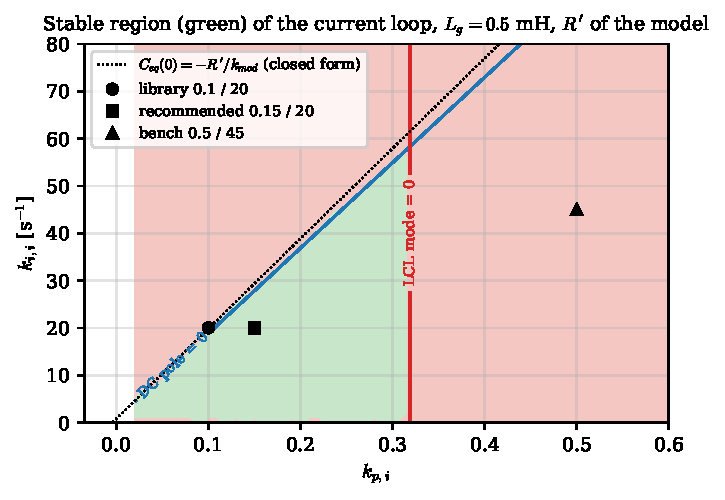
\includegraphics[width=0.72\linewidth]{figures/fig_stability_map.pdf}
\caption{Stable region of the current loop in the plane of the gains ($L_g = \SI{0.5}{mH}$, resistance of the model). The lower boundary is the DC mode (closed form (\ref{eq:dc_condition}) dotted), the right one the LCL mode; the library default lies on the lower boundary, the old bench gains outside the right one.}
\label{fig:stability}
\end{figure}

\subsection{Closed-loop modes and transients}
\label{sec:modes}

Table~\ref{tab:gains} gives the three groups of closed-loop poles: the real DC pole, the LCL mode near \SI{1.4}{kHz} and the pair born from the resonant poles of $\Ceq$ at $\pm\wo$, pulled by the loop to about \SI{64}{Hz} with $\sigma = \SI{-109}{s^{-1}}$ for the recommended gains. The last pair sets the convergence of the fundamental: the envelope of the current error after a reference step settles in about $3/|\sigma| \simeq \SI{30}{ms}$ (the end of the ramp of Fig.~\ref{fig:startup} shows \SI{2}{\percent} of overshoot and no visible tail). A step of the reference of a single-phase current, however, is not a step of a vector: the current cannot jump, the new fundamental starts from the instantaneous value of the old one and the difference is a decaying DC component of the physical current, which the FHT shows as a \SI{50}{Hz} ripple on $i_d$ and $i_q$ until the DC mode has absorbed it. With the DC pole at \SI{-30}{s^{-1}} the \SI{5}{\percent} settling of a $-0.3\pu$ step of $i_q^*$ is \SI{220}{ms} (Fig.~\ref{fig:zoom}, right), far longer than the \SI{30}{ms} of the envelope; the rate limiter on $i_d^*$ (\SI{2}{pu/s}) exists for this reason, a slow ramp producing almost no DC component. The LCL mode, at $\sigma = \SI{-55}{s^{-1}}$, is excited by the enable and by the reference transients and rings for a few tens of milliseconds at \SI{1.4}{kHz} with a small amplitude (Fig.~\ref{fig:gainszoom}).

% =====================================================================================================
\section{Analysis of the PLL}
\label{sec:pll}

\subsection{Virtual quadrature: equivalence with the SOGI-QSG}
\label{sec:sogi}

With the PLL locked, (\ref{eq:virtual_beta}) is again a frequency-shifted linear filter: the low pass $F(s) = 1/(1 + \tau s)$ applied in the synchronous frame to the vector $\vec u = u_g + \jj u_\beta$ is, in the stationary frame, the complex-coefficient filter $F(s - \jj\wo)$, and $u_\beta$ is the imaginary part of its output. Writing $F(s - \jj\wo) = (1 + \tau s + \jj\tau\wo)/[(1 + \tau s)^2 + \tau^2\wo^2]$ and taking the imaginary part of $F(s - \jj\wo)(u_g + \jj u_\beta)$,
\begin{equation}
u_\beta\,[(1 + \tau s)^2 + \tau^2\wo^2] = \tau\wo\,u_g + (1 + \tau s)\,u_\beta
\quad\Longrightarrow\quad
H_\beta(s) = \frac{u_\beta}{u_g} = \frac{k\,\wo^2}{s^2 + k\,\wo s + \wo^2}, \qquad k = \frac{1}{\tau\wo},
\label{eq:sogi}
\end{equation}
exactly the quadrature output of the second-order generalized integrator used as quadrature-signal generator \cite{ciobotaru2006, rodriguez2006}, with the gain $k = 1/(\tau\wo) = 0.5$ for $\tau = 2/\wo$. Its properties follow: $H_\beta(\jj\wo) = -\jj$, i.e. unit gain and exactly \SI{90}{\degree} of lag at the fundamental for any $\tau$; a second-order band pass character with $\zeta = k/2 = 0.25$ and the pole pair at $\sigma = -k\wo/2 = \SI{-78.5}{s^{-1}}$ (time constant \SI{12.7}{ms}: the virtual component settles in about \SI{50}{ms} after a phase jump, Fig.~\ref{fig:sogi}); an attenuation of the harmonics of the terminal voltage, $|H_\beta| = 0.061$ at the third and $0.021$ at the fifth, while the in-phase component is the raw $u_g$; and a DC gain $k = 0.5$, so that a DC offset of the voltage measurement enters $u_\beta$ halved and both components of the virtual vector then carry a term at $-\wo$ in the PLL frame (a \SI{50}{Hz} ripple of $u_\eta$). The choice $k = 0.5$ is on the slow and selective side of the usual range $k = 0.5 \ldots \sqrt2$ \cite{golestan2017}; the double-integrator observer and the low PLL bandwidth make the residual ripple irrelevant, and the settling of the PLL is dominated by the SOGI pair rather than by the loop. In the discrete implementation the filter input is one step behind and $u_\beta$ of the previous step is used (Sect.~\ref{sec:disc_pll}), which adds a lag of one step to the loop of (\ref{eq:sogi}); the simulation shows no visible effect.

\subsection{PLL loop and angle observer}
\label{sec:pllloop}

With $|\vec u| \simeq 1$ the quadrature component is $u_\eta \simeq \sin(\theta_g - \theta) \simeq \theta_g - \theta$, and the loop $\dot\theta = \omega_{nom}(1 + k_{p,pll}u_\eta)$ is of type 1 with the single pole
\begin{equation}
s_{pll} = -k_{p,pll}\,\omega_{nom} = \SI{-314}{s^{-1}} \quad (\SI{3.2}{ms}), \qquad \Delta\theta_{ss} = \frac{\Delta\omega}{k_{p,pll}\,\omega_{nom}} = \SI{1.15}{\degree} \text{ per Hz of frequency offset}:
\label{eq:pll_loop}
\end{equation}
without the integral term ($k_{i,pll} = 0$) a grid frequency off the nominal leaves a static phase error, \SI{1.15}{\degree/Hz}, which the control sees as a rotation of its dq frame: the current then is in phase with the terminal voltage within that angle, a reactive power of $\sin(\SI{1.15}{\degree}) = \SI{2}{\percent}$ per Hz. Within the $\pm\SI{0.5}{Hz}$ of a European grid this is acceptable; a small $k_{i,pll}$ (a few s$^{-1}$) would remove it with a slow integrator and is available in the parameters. The angle is then followed by the double-integrator observer, $\hat x(k+1) = A_o\hat x(k) + L_o\,(\theta - \hat\theta)$ with $A_o = [1\ \ \ts;\ 0\ \ 1]$ and the poles at $\ee^{-\wo\ts}$, $\ee^{-4\wo\ts}$ (continuous equivalents $-314$ and \SI{-1257}{s^{-1}}): it adds no steady-state error (a ramp input is reproduced exactly by the double integrator) and gives the smoothed angle $\hat\theta$ and $\hat\omega$. The whole chain, SOGI pair, PLL pole and observer, responds to a \SI{30}{\degree} phase jump with a peak error of \SI{32}{\degree} and settles within \SI{0.6}{\degree} in \SI{24}{ms}; a \SI{+1}{Hz} step gives the predicted \SI{-1.2}{\degree} of static error and $\hat\omega = 1.02\,\omega_{nom}$ (Fig.~\ref{fig:pllsim}). When locked, $\hat\theta$ lags the grid angle by \SI{2.4}{\degree}, essentially the one control step (\SI{2.25}{\degree}) of the acquisition delay: the dq frame of the control is the frame of the \emph{acquired} voltage, consistently with the acquired current it regulates, so the current is in phase with the actual terminal voltage within \SI{0.7}{\degree} (Sect.~\ref{sec:verification}).

\begin{figure}[htb]
\centering
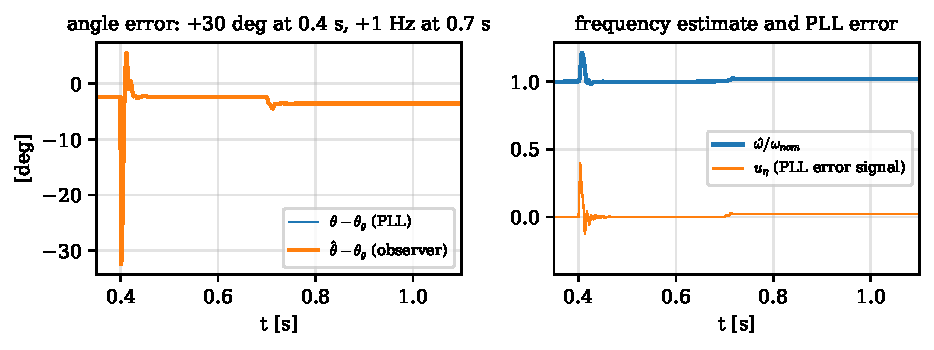
\includegraphics[width=0.95\linewidth]{figures/fig_sim_pll.pdf}
\caption{PLL on the controller as coded (no current reference): angle errors of the PLL ($\theta$) and of the observer ($\hat\theta$) for a \SI{+30}{\degree} phase jump at \SI{0.4}{s} and a \SI{+1}{Hz} frequency step at \SI{0.7}{s} (left); frequency estimate and PLL error signal $u_\eta$ (right). The type-1 loop leaves \SI{1.2}{\degree} of static error per Hz.}
\label{fig:pllsim}
\end{figure}

\begin{figure}[htb]
\centering
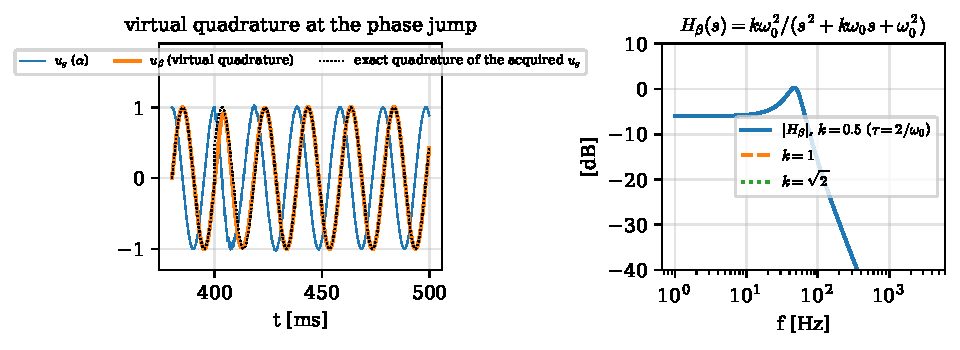
\includegraphics[width=0.95\linewidth]{figures/fig_sim_sogi.pdf}
\caption{Virtual quadrature component at the phase jump against the exact quadrature of the acquired voltage (left) and frequency response (\ref{eq:sogi}) of the equivalent SOGI for $k = 0.5$ (as coded), $1$ and $\sqrt2$ (right).}
\label{fig:sogi}
\end{figure}

% =====================================================================================================
\section{Analysis of the DC-link voltage loop}
\label{sec:dclink}

In mode 1 the plant of the outer loop is the energy balance of the DC link. With the current loop ideal, a current $i_d$ (pu, positive out of the bridge) in phase with the grid voltage $u_{g,pk}$ draws the mean power $P = u_{g,pk}\,i_{bez}\,i_d/2$ from the DC link, so that
\begin{equation}
\frac{\dif u_{dc}}{\dif t} = -K\,i_d + \frac{P_{in}}{C_{dc}\,u_{dc,nom}^2\,u_{dc}}, \qquad K = \frac{u_{g,pk}\,i_{bez}/2}{C_{dc}\,u_{dc,nom}^2} = \SI{26}{s^{-1}} \text{ per pu of } i_d,
\label{eq:dc_plant}
\end{equation}
$u_{dc}$ in per unit of $u_{dc,nom}$ and $P_{in}$ the power fed into the DC link. The sign is the reason for $i_d^* = -y_{udc}$: a positive error (voltage below the reference) must produce a current \emph{into} the bridge. On top of the mean, the instantaneous power of a single-phase converter pulsates at $2f_0$ and the DC-link voltage carries the ripple $\Delta u_{pp} = P/(\wo C_{dc} u_{dc}) = \SI{66}{V}$ peak-peak at \SI{50}{kW} (\SI{8.3}{\percent}; \SI{26}{V} at the \SI{20}{kW} of the simulation), which must not reach the current reference: a \SI{100}{Hz} component of $i_d^*$ is a third harmonic (and a fundamental) of the current, and a DC offset of the current, which pulsates the DC-link power at $f_0$, would be fed back through the loop as a \SI{50}{Hz} component of $i_d^*$, i.e. a DC and a second harmonic of the current. The measurement filter is therefore the moving average over one grid period ($N = 2\pi/(\wo\ts) = 160$ samples), $H_{ma}(z) = (1 - z^{-N})/[N(1 - z^{-1})]$, with exact zeros at every multiple of \SI{50}{Hz} and a group delay of $(N - 1)\ts/2 = \SI{9.9}{ms}$ \cite{golestan2014}. The loop is
\begin{equation}
L_{dc}(s) = \left(\kpu + \frac{\kiu}{s}\right)\frac{1}{1 + s/\omega_{c,i}}\,\frac{K}{s}\,H_{ma}(s)\,\ee^{-s\ts}, \qquad \omega_{c,dc} \simeq \kpu K = \SI{52}{rad/s} \ (\SI{8.3}{Hz}),
\label{eq:dc_loop}
\end{equation}
the inner loop represented by a lag at its crossover $\omega_{c,i} = \SI{705}{rad/s}$. At the crossover (\SI{50.7}{rad/s} exact) the moving average costs \SI{29}{\degree}, the PI zero at $\kiu/\kpu = \SI{10}{rad/s}$ \SI{11}{\degree} and the inner loop \SI{4}{\degree}: $\varphi_m = \SI{45.5}{\degree}$ (Fig.~\ref{fig:dcloop}), against \SI{75}{\degree} without filter, where however the loop gain at \SI{100}{Hz} is $0.062$ and at \SI{50}{Hz} $0.15$. A first-order low pass of \SI{5}{ms} in place of the average would leave \SI{60}{\degree} of margin and $0.019$ of gain at \SI{100}{Hz}: a ripple of $7\cdot10^{-3}\pu$ rms on $i_d^*$ against $0.02\cdot10^{-3}$ with the average (Fig.~\ref{fig:dcsim}). The step response of the loop is set by its \SI{8}{Hz} bandwidth: a step of \SI{20}{kW} (\SI{40}{\percent}) of input power charges the DC link by about $P/(\omega_{c,dc}\,C_{dc}\,u_{dc}) \simeq \SI{165}{V}$ before the current catches up (\SI{163}{V} in the simulation), and the average voltage is back within \SI{2}{\percent} of the excursion in \SI{340}{ms}. The gains are a conservative starting point (the comment of the parameter file says so): a faster loop would need a smaller $C_{dc}$ swing or a feed-forward of the input power, both outside the present implementation.

\paragraph{Third harmonic from the feed-forward.} With the moving average the current reference is clean, yet the current carries a third harmonic of \SI{1.26}{\percent} of the fundamental in the simulation at \SI{20}{kW}, against \SI{0.23}{\percent} with the low pass that lets the ripple through. The origin is not the loop but the DC-link feed-forward (\ref{eq:ff}): the division uses the sample of the \emph{previous} trigger, and on the \SI{100}{Hz} ripple of amplitude $1.65$\,\% one step of delay leaves the error $2\sin(2\wo\ts/2) = \SI{7.9}{\percent}$ of the ripple, $0.13$\,\% of the bridge voltage, which multiplied by the fundamental of the modulation index gives a third harmonic (and a fundamental) of the bridge voltage: $0.0044\pu$ of third-harmonic current through $3\wo(L_c' + L_g')$, against $0.0050\pu$ measured. Using the sample of the same trigger in an experiment of the script lowers the harmonic to \SI{0.43}{\percent} (the hold still averages over half a step); with the low pass the \SI{100}{Hz} component that reaches $i_d^*$ happens to compensate part of the feed-forward error, which is a coincidence and not a design. A one-step prediction of $u_{dc}$ in the feed-forward (from the previous samples, or from the known ripple model) would remove the harmonic; it is not implemented and the figure is in any case within the usual limits.

\begin{figure}[htb]
\centering
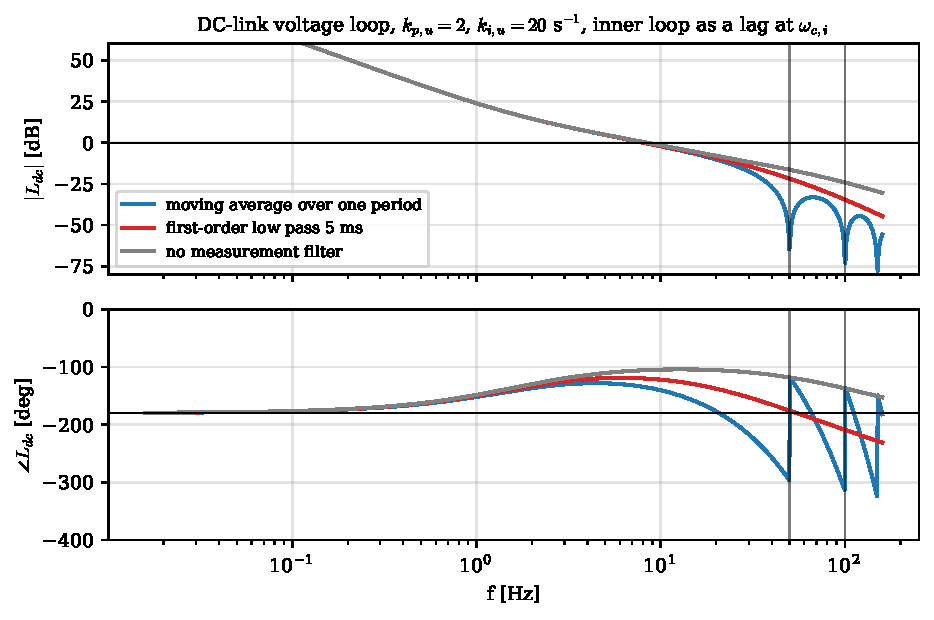
\includegraphics[width=0.9\linewidth]{figures/fig_dclink_loop.pdf}
\caption{Open-loop gain of the DC-link voltage loop (\ref{eq:dc_loop}) with the moving average over one grid period, with a first-order low pass of \SI{5}{ms} and without measurement filter. The average costs \SI{29}{\degree} at the crossover and puts exact zeros at \SI{50}{Hz} and \SI{100}{Hz}.}
\label{fig:dcloop}
\end{figure}

% =====================================================================================================
\section{Discrete-time implementation}
\label{sec:discrete}

\subsection{One control step}
\label{sec:step}

The function runs every $\tc$ and executes the control on the rising edge of the TRGO. On a control step, with the states indexed by $k$ (values at the beginning of the step, a bar for the value after the update), the operations are, in the order of the code:
\begin{enumerate}
\item \textbf{Acquisitions:} $i_s$, $u_{ac}$, $u_{dc}$ (and $u_{dc,p}$, $u_{dc,n}$) of the previous trigger are read; the present samples are quantized, $x_q = q\,\mathrm{round}(x/q)$ with $q = 2^{-11}\pu$, the current with the optional noise added before the quantizer, and stored for the next step. At the first trigger the DC-link filters and the moving-average buffer are initialized with the measured voltage.
\item \textbf{Clock alignment:} PI on $t_{master} - t_{loc}$ with back-calculation anti-windup, correction applied from the next step (zero gains by default).
\item \textbf{PLL} (Sect.~\ref{sec:disc_pll}): $u_g = u_{ac}/u_{g,nom}$; $\theta = \theta(k)$ is the angle of this step; the low passes are updated with the inputs of the previous step, $x_f \leftarrow a\,x_{in}(k-1) + (1 - a)\,x_f$ with $a = \ts/\tau$; $u_\beta = x_{\xi f}\sin\theta + x_{\eta f}\cos\theta$; $u_\xi = u_g\cos\theta + u_\beta\sin\theta$, $u_\eta = -u_g\sin\theta + u_\beta\cos\theta$, stored as the filter inputs of the next step; PI on $u_\eta$ with the limit $\pm 2$ and back-calculation; $\theta(k+1) = \theta + \omega_{nom}\ts(1 + y_{pll}) \bmod 2\pi$; observer: $\hat\theta = \hat x_1(k)$, $\hat\omega = \hat x_2(k)$, $e = \theta - \hat\theta$ wrapped, $\bar{\hat x}_1 = \hat x_1 + \ts\hat x_2 + l_1 e$ (wrapped), $\bar{\hat x}_2 = \hat x_2 + l_2 e$.
\item \textbf{FHT} (Sect.~\ref{sec:disc_fht}): $\ihat_\alpha = \hat x_1(k)$, $\ihat_\beta = -\hat x_2(k)/\wo$ (both from the state \emph{before} the update); $e = i_s - \hat x_1(k)$; $\bar{\hat x} = A_d\hat x(k) + L_d\,e$ with $A_d = I + A\ts$. Then (\ref{eq:dq}) with $\hat\theta$.
\item \textbf{References:} mode 0, rate limiter $|\Delta i_d^*| \le \dot\imath_{max}\ts$ towards the target ($i_{ref}$ from $t_{ref}$, zero before the enable); mode 1, reference low pass $\bar u^*_{dc,f} = u^*_{dc,f} + (\ts/\tau_{ref})(u_{dc}^* - u^*_{dc,f})$, moving average of the acquired $u_{dc}$ over the last $N$ samples (circular buffer), optional low pass, PI with the limit $\pm i_{lim}$ and back-calculation, $i_d^* = -y_{sat}$ (integrator reset while disabled or slave).
\item \textbf{Current PI} (Sect.~\ref{sec:disc_pi}): with the clip flag of the previous step, per axis $\bar x = x + \kii\ts\,e$ and $y = \kpi e + \bar x$ (or $\bar x = (1 - c_{rel}\ts)x$, $y = \kpi e + x$ while clipped); $m_{d,q} = y_{d,q}/\max(u_{dc}, u_{dc,min})$ with the \emph{acquired} $u_{dc}$ of the previous trigger; circular limiter of radius $u_{lim}$ and clip flag for the next step. Before the enable the states are zero; at the first enabled step they are pre-loaded with (\ref{eq:bumpless}); a slave takes $(m_d, m_q)$ from \code{sync}.
\item \textbf{Modulation index:} $m = m_d\cos\hat\theta - m_q\sin\hat\theta$, held until the next trigger; the log and the \code{sync} output are updated.
\end{enumerate}
Every $\tc$ the gate commands are computed from the held $m$, saturated in $[m_{low}, m_{up}]$, and the carrier (Sect.~\ref{sec:modulator}).

\subsection{PI integrators}
\label{sec:disc_pi}

The vector PI is coded with the integrator state updated before the output,
\begin{equation}
\bar x = x(k) + \kii\ts\,e(k), \qquad y(k) = \kpi\,e(k) + \bar x, \qquad C(z) = \kpi + \kii\ts\,\frac{z}{z - 1},
\label{eq:pi_code}
\end{equation}
a backward Euler integrator; while the clip flag of the previous step is set, $\bar x = (1 - c_{rel}\ts)\,x(k)$ and the output uses the held state. No exactness is required here: the integrator pole is at $z = 1$ with any method, which is all the dq regulation needs, and the equivalent stationary-frame controller (\ref{eq:ceq_z}) has its resonant poles at exactly $\ee^{\pm\jj\wo\ts}$ whatever the integrator form, because the frame rotations are exact. The approximation only moves the controller zero by a phase of $\omega\ts/2$ (\SI{2.5}{\degree} at the crossover), immaterial for the margins. The PLL and DC-link PIs use the same update with back-calculation.

\subsection{Acquisition delay and DC-link feed-forward}
\label{sec:disc_ff}

The one-step delay of the samples is part of the plant delay (\ref{eq:delay}) and is included as such in the design; it also affects two feed-forward paths. The DC-link feed-forward divides by the $u_{dc}$ sample of the previous trigger: on a slowly varying DC-link voltage the compensation is exact, on the \SI{100}{Hz} ripple of the single-phase DC link it leaves the residual of Sect.~\ref{sec:dclink} (a third harmonic of \SI{1.3}{\percent} of the fundamental at \SI{20}{kW}); a one-step prediction of $u_{dc}$ would remove it. The bumpless start (\ref{eq:bumpless}) pre-loads the integrators with the acquired terminal voltage rotated by $1.5\,\hat\omega\ts$ (one step of acquisition delay plus half a step of hold), so that the bridge voltage at the first switching half-period matches the grid voltage \emph{of that half-period}: the residual inrush is zero within the quantization (\SI{0.000}{pu} peak in the simulation, Fig.~\ref{fig:zoom}).

\subsection{PLL: low passes, feedback of the virtual component and observer}
\label{sec:disc_pll}

The two low passes of the PLL are coded as $y(k) = a\,x(k-1) + (1 - a)\,y(k-1)$, $a = \ts/\tau = 0.0196$: a forward Euler integrator with the input one step behind, i.e. $F(z) = a z^{-1}/(1 - (1 - a)z^{-1})$, a lag of one step more than the continuous filter; the virtual $u_\beta$ is computed from the filter outputs of this step and the angle of this step, and the rotations use $\theta(k)$, the PLL angle before its update. The equivalence (\ref{eq:sogi}) therefore holds with an extra $z^{-1}$ in the loop of the virtual component, which moves the SOGI pair by less than \SI{3}{\percent} and leaves $H_\beta(\ee^{\jj\wo\ts})$ within \SI{1}{\degree} of $-\jj$: the locked PLL frame lags the grid angle by the acquisition step only (\SI{2.4}{\degree} measured against \SI{2.25}{\degree}, Sect.~\ref{sec:pllloop}). The angle increment $\omega_{nom}\ts(1 + y_{pll})$ and the wrap to $[-\pi, \pi)$ are exact; the observer gains are those of the forward Euler model of the double integrator, which is the exact discretization of $\ddot\theta = 0$ ($A_o = [1\ \ \ts;\ 0\ \ 1]$ is $\ee^{A\ts}$): the observer poles are exactly at $\ee^{-\wo\ts}$ and $\ee^{-4\wo\ts}$, $l_1 = 2 - \ee^{-\wo\ts} - \ee^{-4\wo\ts} = 0.1839$, $l_2 = [\ee^{-5\wo\ts} - (1 - l_1)]/\ts = \SI{44.78}{s^{-1}}$.

\subsection{FHT: internal model, gains and output timing}
\label{sec:disc_fht}

The FHT is coded with the forward Euler matrix of the oscillator (\ref{eq:fht_model}), as the Simulink block of the bench,
\begin{equation}
A_d = I + A\ts = \begin{bmatrix} 1 & \ts \\ -\wo^2\ts & 1 - \delta\wo\ts \end{bmatrix}, \qquad
\bar{\hat x} = A_d\,\hat x(k) + L_d\,[i_s(k-1) - \hat x_1(k)], \qquad L_d = \begin{bmatrix} l_1 \\ l_2 \end{bmatrix},
\label{eq:fht_code}
\end{equation}
with the gains placed in closed form on the same matrix so that the observer poles are exactly at $\ee^{-\wo\ts}$ and $\ee^{-4\wo\ts}$ ($l_1 = 2 - \delta\wo\ts - \ee^{-\wo\ts} - \ee^{-4\wo\ts} = 0.1819$, $l_2 = [\ee^{-5\wo\ts} - (1 - l_1)(1 - \delta\wo\ts) - \wo^2\ts^2]/\ts = \SI{29.59}{s^{-1}}$, function \code{fht\_gains} of the parameter file). The forward Euler oscillator by itself has its eigenvalues outside the unit circle ($|z|^2 = (1 - \delta\wo\ts)^2 + \wo^2\ts^2$ for small $\delta$), but here the matrix is inside an observer whose poles are placed by $L_d$: the stability of the tracker is not in question, only the exactness of the tracking at $\wo$, which requires the \emph{internal model} to generate the sampled sinusoid, i.e. the eigenvalues of $A_d$ at $\ee^{\pm\jj\wo\ts}$. Table~\ref{tab:fhtvar} compares the coded form with two alternatives, computing in each case the response from the acquired sample to the estimates used in the step (the state before the update, which lags the sample by one step). The coded form, with $\delta = 0.05$, gives $\Hu(\ee^{\jj\wo\ts}) = 0.998\,\angle\SI{-0.06}{\degree}$ and $\Hv = 0.994\,\angle\SI{-88.5}{\degree}$: the forward Euler matrix, whose eigenvalues have a modulus above one and an angle slightly below $\wo\ts$, happens to compensate most of the lag of the damping and of the one-step output timing, so the tracking is exact within \SI{0.2}{\percent} and \SI{1.5}{\degree}. The exact rotation matrix with $\delta = 0$,
\begin{equation}
\ee^{A\ts} = \begin{bmatrix} \cos\wo\ts & \sin(\wo\ts)/\wo \\ -\wo\sin\wo\ts & \cos\wo\ts \end{bmatrix},
\label{eq:fht_exact}
\end{equation}
gives $\Hu = 1$, $\Hv = -\jj$ exactly from the acquired sample to the estimates \emph{after} the update, and $1\,\angle\SI{0}{\degree}$, $1\,\angle\SI{-90}{\degree}$ from the sample to the estimates used (the one-step lag of the output cancels against the lead of the observer, as in the coded form): it costs the same two multiplications and is the form to use if the tracker is rewritten; the gain error of the coded form is small enough that the regulated fundamental is within \SI{0.4}{\percent} of its reference (Sect.~\ref{sec:verification}). What the discretization does not change is the DC leakage: $\Hu(1) = 0.7245$ and $\Hv(1) = 1.28$ in all three variants (the observer gains, not the matrix, set the DC response), and so the DC mode of Sect.~\ref{sec:dcmode}; nor the attenuation at the LCL resonance, $|\Hu| = 0.185$ in all three.

\begin{table}[htb]
\centering\small
\caption{Discrete FHT variants with the poles placed at $\ee^{-\wo\ts}$, $\ee^{-4\wo\ts}$: response from the acquired sample to the estimates used in the step at the fundamental and at DC, and attenuation at the LCL resonance.}
\label{tab:fhtvar}
\begin{tabular}{@{}lccccc@{}}
\toprule
internal model & $l_1$, $l_2$ [s$^{-1}$] & $\Hu(\ee^{\jj\wo\ts})$ & $\Hv(\ee^{\jj\wo\ts})$ & $\Hu(1)$, $\Hv(1)$ & $|\Hu(\ee^{\jj\wres\ts})|$ \\
\midrule
forward Euler, $\delta = 0.05$ (as coded) & 0.1819, 29.59 & $0.998\,\angle\SI{-0.06}{\degree}$ & $0.994\,\angle\SI{-88.5}{\degree}$ & 0.725, 1.276 & 0.185 \\
forward Euler, $\delta = 0$ & 0.1839, 32.45 & $1.006\,\angle\SI{+0.21}{\degree}$ & $1.024\,\angle\SI{-90.4}{\degree}$ & 0.725, 1.290 & 0.187 \\
exact rotation (\ref{eq:fht_exact}), $\delta = 0$ & 0.1823, 31.33 & $1.000\,\angle\SI{0}{\degree}$ & $1.000\,\angle\SI{-90}{\degree}$ & 0.725, 1.265 & 0.185 \\
\bottomrule
\end{tabular}
\end{table}

\subsection{Modulator}
\label{sec:modulator}

Every $\tc$ the carrier is $r = \arcsin[\sin(2\pi f_{pwm}t_{loc} - \phi - \pi/2)]/\pi + 1/2$, a triangle between 0 and 1, and the TRGO flag is set when $r \le 2f_{pwm}\tc$ (bottom) or $r \ge 1 - 2f_{pwm}\tc$ (top, double update). The gate commands of leg $u$ with the reference $m \in [-1, 1]$ and the dead time $d = t_{dead}f_{pwm}$ as a fraction of the carrier period are: for $m \ge 0$, $Q_2$ on (the neutral path ready), $Q_1$ on while $r < m - d$ (duty $m$), $Q_3$ on while $r \ge m + d$; for $m < 0$, $Q_3$ on, $Q_4$ on while $r > 1 + m + d$ (duty $-m$), $Q_2$ on while $r \le 1 + m - d$. Leg $v$ uses $-m$ on the same carrier (Fig.~\ref{fig:modulator}). The leg voltage against the neutral point is $+u_{dc}/2$ with $Q_1$ on, $-u_{dc}/2$ with $Q_4$ on and $0$ otherwise; the switching instants are quantized to $\tc$, so with $\tc = \SI{500}{ns}$ the \SI{300}{ns} dead time becomes 0 or \SI{500}{ns} (use \SI{100}{ns} for the losses). The gates are off until the first control step with $t \ge t_{enable}$, and follow the enable state of the last control step. Differences from the Simulink diagram of the bench: no $1/(\tc s + 1)$ filters on the modulation index, no blanking of the neutral switch at the carrier extremes, the PLL reads the terminal voltage of the block (the bench model read the line EMF), and no device model (the switches are resistive, $R_{on}$ only).

\begin{figure}[htb]
\centering
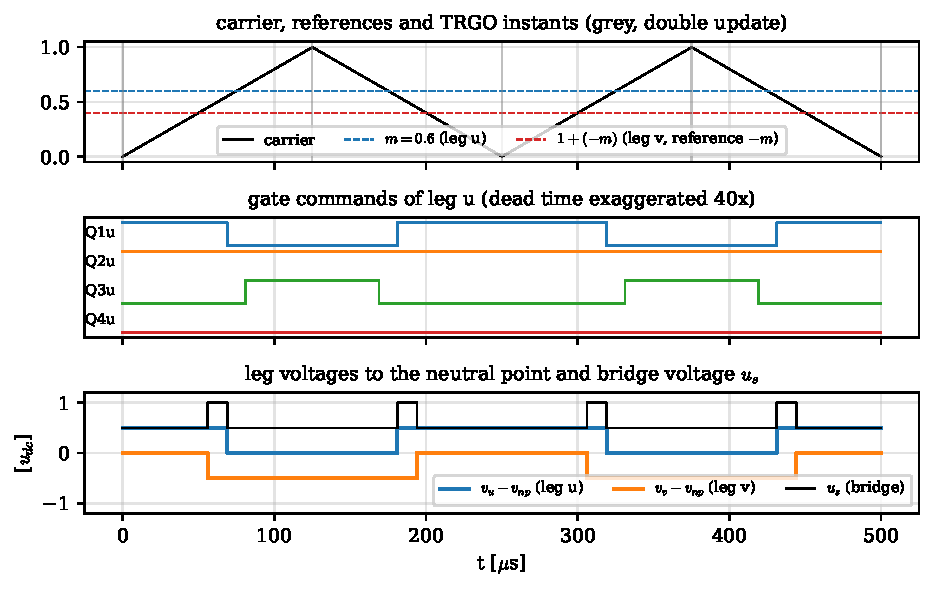
\includegraphics[width=0.9\linewidth]{figures/fig_modulator.pdf}
\caption{Three-level modulation of one carrier period ($m = 0.6$): carrier, references of the two legs and TRGO instants (top), gate commands of leg $u$ with the dead time exaggerated (centre), leg voltages against the neutral point and bridge voltage, three levels per leg and five on the bridge at $2f_{pwm}$ (bottom).}
\label{fig:modulator}
\end{figure}

\subsection{Summary}

\begin{table}[htb]
\centering\small
\caption{Discretization of the controller: form used and what exactness buys.}
\label{tab:summary}
\begin{tabular}{@{}R{3.4cm}R{4.6cm}R{1.5cm}R{6.2cm}@{}}
\toprule
operation & form in \code{afe\_sp\_ttype\_ctrl\_pwm} & exact needed & consequence of an approximate form \\
\midrule
PLL angle, frame rotations & constant increment modulo $2\pi$, trigonometric functions & yes (by construction) & the resonant poles of $\Ceq(z)$ sit at exactly $\ee^{\pm\jj\wo\ts}$ for any PI form \\
PI integrators (current, PLL, DC link, clock) & backward Euler, state updated before the output & no & pole at $z = 1$ with any method; zero moved by $\omega\ts/2$ \\
FHT internal model & forward Euler, $\delta = 0.05$, gains placed on the same matrix & practically & tracking exact within 0.2\,\% and \SI{1.5}{\degree} as coded; the exact rotation with $\delta = 0$ costs the same; DC leakage and resonance attenuation unchanged \\
FHT output timing & both outputs from the state before the update & -- & consistent pair; the one-step lag cancels the observer lead at $\wo$ \\
virtual quadrature of the PLL & forward Euler low passes with the input one step behind & no & SOGI pair moved by $< 3$\,\%, $H_\beta(\wo)$ within \SI{1}{\degree} of $-\jj$ \\
DC-link feed-forward & division by the sample of the previous trigger & -- & third harmonic of 1.3\,\% at \SI{20}{kW} from the \SI{100}{Hz} ripple; a one-step prediction would remove it \\
moving average of $u_{dc}$ & circular buffer of $N = 160$ samples & -- & exact zeros at the multiples of \SI{50}{Hz} only if $N\ts$ is one grid period \\
modulator & gates every $\tc$, instants quantized to $\tc$ & -- & dead time 0 or \SI{500}{ns} with $\tc = \SI{500}{ns}$ \\
\bottomrule
\end{tabular}
\end{table}

% =====================================================================================================
\section{Numerical verification}
\label{sec:verification}

The companion script simulates the controller as coded (acquisitions with quantizer, noise and one-step delay, PLL, FHT, references, PI with feed-forward and limiter, modulation index held over the step) on the average model of the power stage, the plant (\ref{eq:plant}) driven by $m\,u_{dc}$ with the grid EMF, integrated exactly over each control step; before the enable the bridge is open. The switching ripple is not represented; the modulator is checked separately (Fig.~\ref{fig:modulator}). Table~\ref{tab:sim} collects the results, Figs.~\ref{fig:startup} to \ref{fig:dczoom} the waveforms.

\begin{table}[htb]
\centering\small\setlength{\tabcolsep}{4pt}
\caption{Sampled-data simulation of the controller as coded (noise $0.01\pu$ rms on the current sample, quantizer $2^{-11}$).}
\label{tab:sim}
\begin{tabular}{@{}R{6.2cm}R{9.6cm}@{}}
\toprule
test & result \\
\midrule
enable at \SI{0.1}{s} with the PLL locked, $\kpi = 0.15$ & bumpless: peak current \SI{0.000}{pu} in the first \SI{60}{ms}, DC component $-0.0002\pu$ after \SI{100}{ms} \\
ramp $0 \to 1\pu$ of $i_d^*$ from \SI{0.35}{s}, \SI{2}{pu/s} & no overshoot of the envelope beyond \SI{2}{\percent}; at \SI{1}{pu}: FHT estimates $i_d = 1.0000$, $i_q = 0.0000$; actual fundamental $1.004\pu\,\angle\SI{1.98}{\degree}$ on the EMF, terminal voltage $0.786\pu\,\angle\SI{2.72}{\degree}$: current in phase with the terminal voltage within \SI{0.7}{\degree}; $m_d = 0.706$, $m_q = 0.075$; DC $-2\cdot10^{-5}\pu$ \\
step $i_q^*$: $0 \to -0.3\pu$ at \SI{1.0}{s} & \SI{5}{\percent} settling of the FHT estimate in \SI{220}{ms} (DC mode of the single-phase current, \SI{50}{Hz} ripple on $i_d$, $i_q$); residual ripple of $i_q$ $10\cdot10^{-3}\pu$ rms (the noise) \\
same run, library gains $0.1/20$ & identical waveform up to \SI{1.3}{s} (the DC mode at \SI{+5}{s^{-1}} is seeded by noise only: DC component below $10^{-3}\pu$) \\
same run, old bench gains $0.5/45$ & LCL mode unstable: current to the limiter within \SI{60}{ms} of the enable, \SI{40}{\percent} of the steps clipped, peak \SI{11.9}{pu}, DC component \SI{1.2}{pu} after the ramp \\
DC step of \SI{0.01}{pu} on the bridge voltage at \SI{0.6}{s}, no reference & $\kpi = 0.15$: DC current $+0.277\pu$ (prediction $u_0/[R'(1 + L(0))] = 0.29\pu$); $\kpi = 0.1$: the DC current grows with the time constant of the unstable mode until the modulation limiter stops it at \SI{2.36}{pu} \\
PLL: \SI{+30}{\degree} at \SI{0.4}{s}, \SI{+1}{Hz} at \SI{0.7}{s} & locked error \SI{-2.37}{\degree} (one step is \SI{2.25}{\degree}); jump: peak \SI{32.4}{\degree}, within \SI{0.6}{\degree} after \SI{24}{ms}; frequency: static error \SI{-3.56}{\degree} ($-1.19$ against \SI{-1.15}{\degree/Hz} predicted), $\hat\omega = 1.0200\pu$ \\
mode 1: \SI{20}{kW} step of input power at \SI{0.4}{s}, $C_{dc} = \SI{3}{mF}$ & moving average: $u_{dc}$ peak \SI{+163}{V}, back within \SI{2}{\percent} in \SI{338}{ms}, $i_d^* = -0.397\pu$, ripple of $i_d^*$ $0.02\cdot10^{-3}\pu$ rms, third harmonic of $i_s$ \SI{1.26}{\percent} (feed-forward delay); low pass \SI{5}{ms}: peak \SI{+139}{V}, ripple of $i_d^*$ $7.2\cdot10^{-3}\pu$ rms, third harmonic \SI{0.23}{\percent}; same-trigger feed-forward (experiment): \SI{0.43}{\percent} \\
\bottomrule
\end{tabular}
\end{table}

\begin{figure}[htbp]
\centering
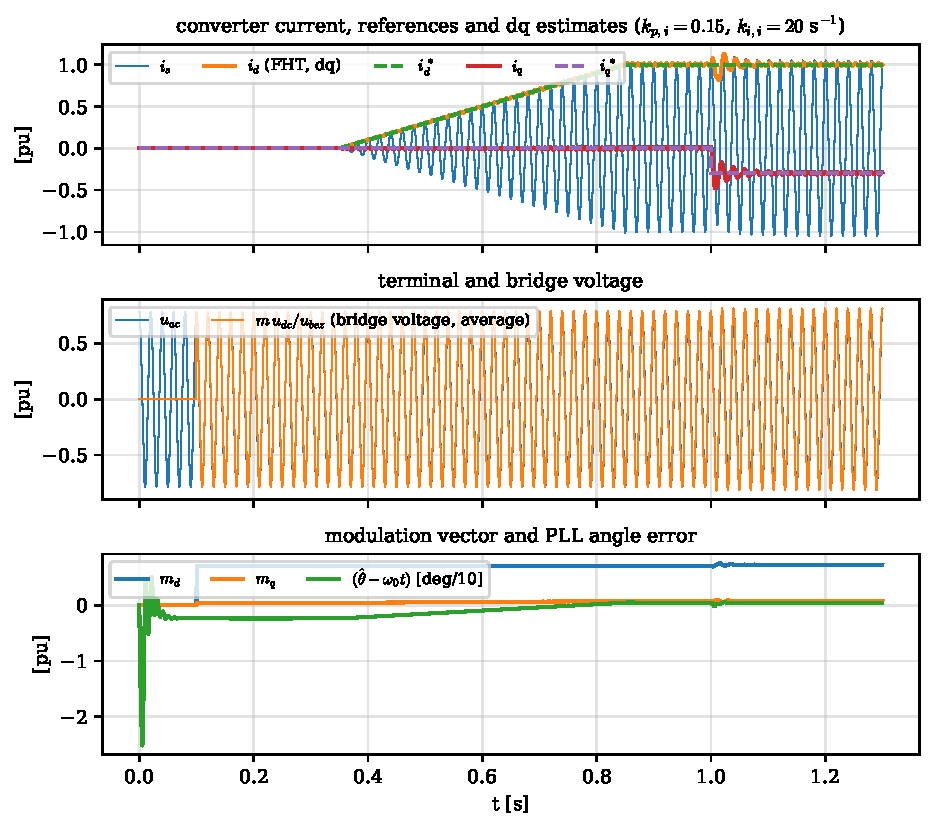
\includegraphics[width=0.95\linewidth]{figures/fig_sim_startup.pdf}
\caption{Start-up with the recommended gains: enable at \SI{0.1}{s}, ramp of $i_d^*$ from \SI{0.35}{s}, step of $i_q^*$ at \SI{1.0}{s}. Converter current with the FHT estimates and the references (top), terminal and average bridge voltage (centre), modulation vector and angle error of the PLL (bottom).}
\label{fig:startup}
\end{figure}

\begin{figure}[htbp]
\centering
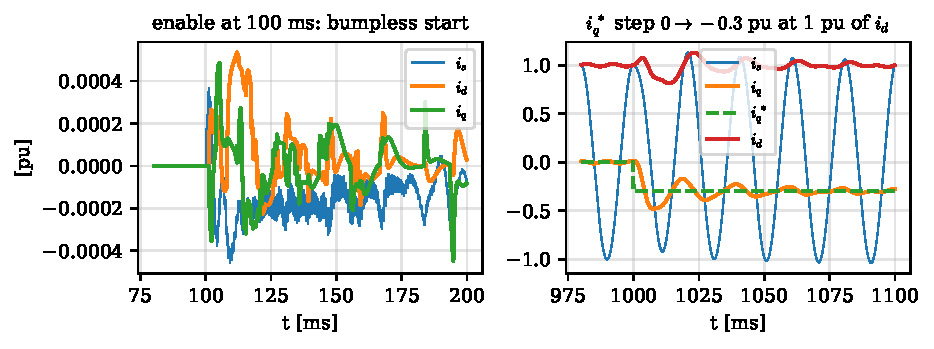
\includegraphics[width=0.95\linewidth]{figures/fig_sim_zoom.pdf}
\caption{Left: the enable at \SI{100}{ms}, bumpless (the bridge starts at the grid voltage). Right: the $-0.3\pu$ step of $i_q^*$ at \SI{1}{pu} of $i_d$; the DC component of the single-phase current appears as a \SI{50}{Hz} ripple on the estimates and decays with the DC mode (\SI{-30}{s^{-1}}).}
\label{fig:zoom}
\end{figure}

\begin{figure}[htbp]
\centering
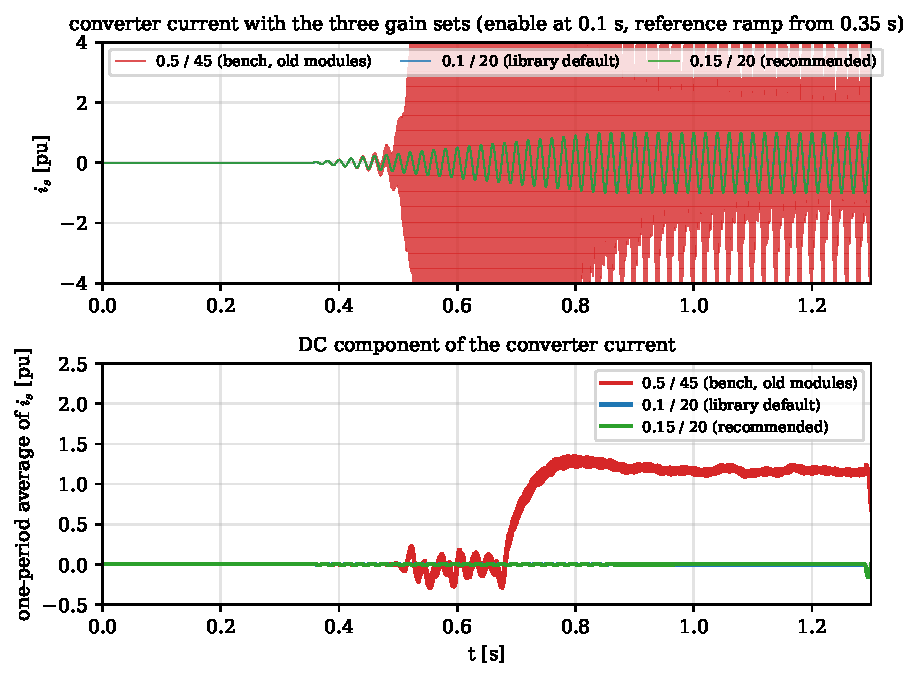
\includegraphics[width=0.95\linewidth]{figures/fig_sim_gains.pdf}
\caption{The same run with the three gain sets: converter current (top) and its one-period average (bottom). The library and the recommended gains give the same waveform; the old bench gains are unstable at the LCL resonance and end up clipped with a DC component.}
\label{fig:gains}
\end{figure}

\begin{figure}[htbp]
\centering
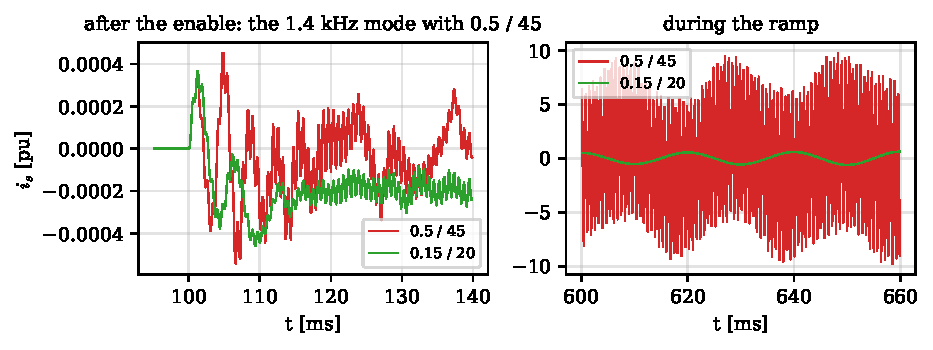
\includegraphics[width=0.95\linewidth]{figures/fig_sim_gains_zoom.pdf}
\caption{Zoom of Fig.~\ref{fig:gains}: the \SI{1.4}{kHz} mode after the enable with the old bench gains against the recommended ones (left) and during the ramp (right).}
\label{fig:gainszoom}
\end{figure}

\begin{figure}[htbp]
\centering
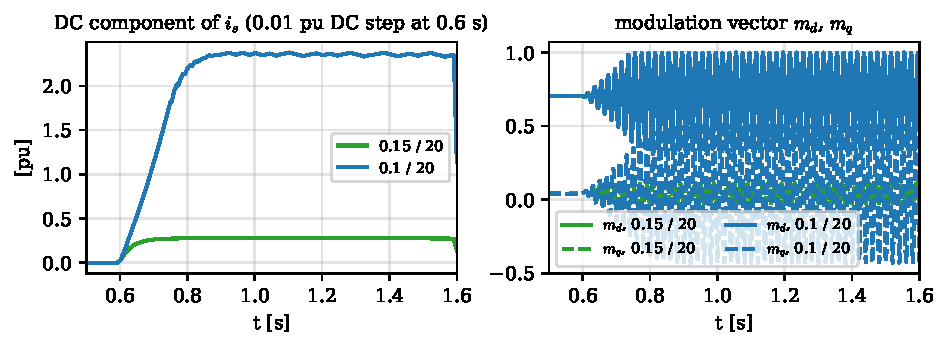
\includegraphics[width=0.95\linewidth]{figures/fig_sim_dcoffset.pdf}
\caption{DC step of \SI{0.01}{pu} on the bridge voltage at \SI{0.6}{s} with no current reference: one-period average of the current (left) and modulation vector (right), where the DC current turns at $-\wo$. Recommended gains: \SI{0.28}{pu} of DC current; library gains: the unstable DC mode runs into the limiter.}
\label{fig:dcoffset}
\end{figure}

\begin{figure}[htbp]
\centering
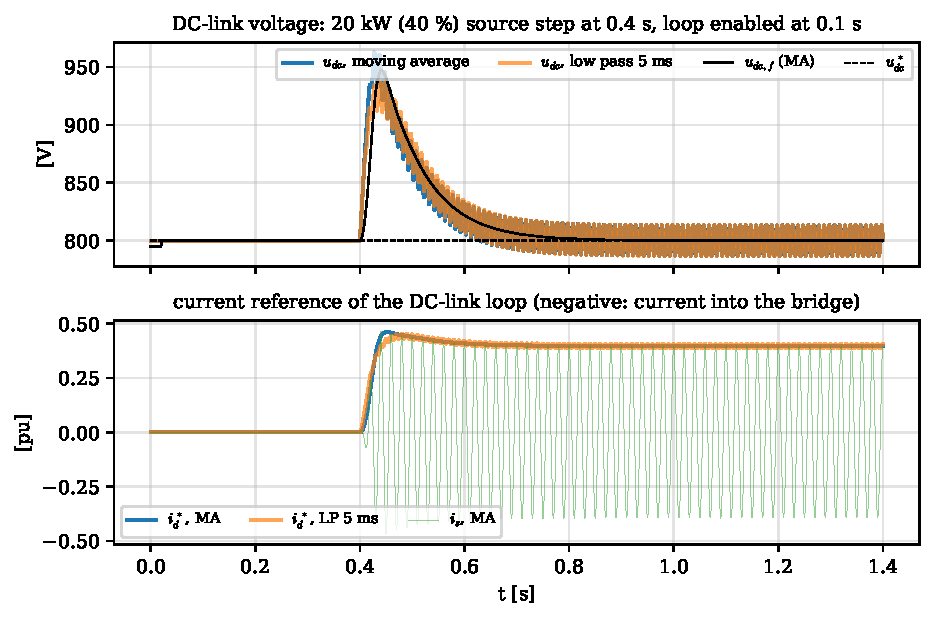
\includegraphics[width=0.95\linewidth]{figures/fig_sim_dclink.pdf}
\caption{Mode 1: DC-link voltage (top) and current reference (bottom) for a \SI{20}{kW} step of input power at \SI{0.4}{s}, with the moving average and with a \SI{5}{ms} low pass on the measurement.}
\label{fig:dcsim}
\end{figure}

\begin{figure}[htbp]
\centering
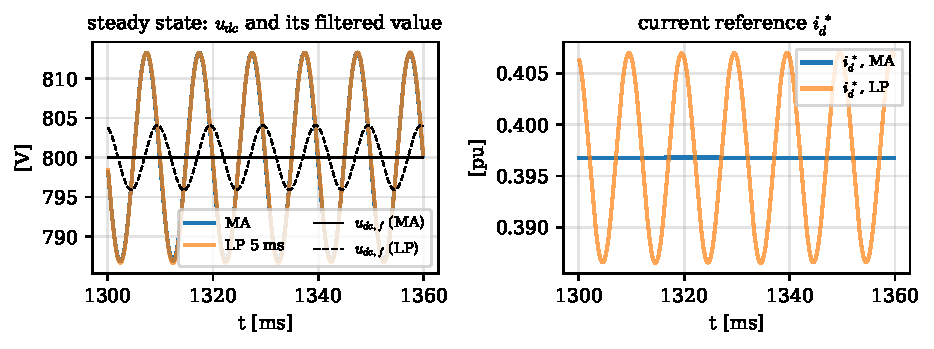
\includegraphics[width=0.95\linewidth]{figures/fig_sim_dclink_zoom.pdf}
\caption{Steady state of Fig.~\ref{fig:dcsim}: \SI{100}{Hz} ripple of the DC-link voltage with the filtered measurements (left) and current reference (right); the low pass lets a \SI{100}{Hz} ripple of $7\cdot10^{-3}\pu$ rms through, the moving average none.}
\label{fig:dczoom}
\end{figure}

% =====================================================================================================
\clearpage
\section{Parameters}
\label{sec:parameters}

\begin{table}[htb]
\centering\footnotesize\setlength{\tabcolsep}{3pt}
\caption{Parameters of the block (\code{afe\_single\_phase\_ttype\_param\_example.m}, struct \code{p}; per unit of the converter base). The recommended current gains are in brackets.}
\label{tab:param}
\begin{tabular}{@{}llll@{}}
\toprule
 & field & value & note \\
\midrule
power stage & \code{p.hw.L1, L2, R1, R2} & \SI{250}{\micro H}, \SI{2}{m\ohm} each & $L_c = \SI{500}{\micro H}$ \\
 & \code{p.hw.Cf, Rcf} & \SI{50}{\micro F}, \SI{50}{m\ohm} & LC \SI{1.0}{kHz}, LCL \SI{1.4}{kHz} \\
 & \code{p.hw.Cdc1, Cdc2, Rdc1, Rdc2} & \SI{6}{mF}, \SI{0.5}{m\ohm} & \SI{3}{mF} in series \\
 & \code{p.hw.Ron, Vth, Goff} & \SI{6}{m\ohm}, \SI{2.5}{V}, \SI{1e-6}{S} & conduction only \\
 & \code{p.hw.ubez, ibez, udc\_nom} & \SI{720}{V}, \SI{177.5}{A}, \SI{800}{V} & bases \\
carrier and gates & \code{p.pwm.fpwm, double\_update, tc} & \SI{4}{kHz}, 1, \SI{500}{ns} & $\ts = \SI{125}{\micro s}$ \\
 & \code{p.pwm.dead\_time, gate\_on, gate\_off} & \SI{300}{ns}, \SI{15}{V}, \SI{-10}{V} & \\
 & \code{p.pwm.m\_up, m\_low, t\_enable, phase} & 1, $-1$, \SI{0.1}{s}, 0 & \\
acquisitions & \code{p.ctrl.adc\_q, i\_noise\_std} & $2^{-11}$, \SI{0.01}{pu} & \\
PLL & \code{p.ctrl.omega\_nom, ug\_nom} & $2\pi\cdot50$, 0.7825 & \\
 & \code{p.ctrl.pll\_kp, pll\_ki, pll\_lim, pll\_tau} & 1, 0, 2, $2/\wo$ & SOGI $k = 0.5$ \\
 & \code{p.ctrl.obs\_l1, obs\_l2} & 0.1839, \SI{44.78}{s^{-1}} & poles $\ee^{[-1\ -4]\wo\ts}$ \\
FHT & \code{p.ctrl.fht\_omega, fht\_delta} & $\wo$, 0.05 & \\
 & \code{p.ctrl.fht\_l1, fht\_l2} & 0.1819, \SI{29.59}{s^{-1}} & poles $\ee^{[-1\ -4]\wo\ts}$ \\
references & \code{p.ctrl.mode, slave} & 0, 0 & \\
 & \code{p.ctrl.i\_ref, t\_ref, i\_ref\_slew, iq\_ref} & \SI{1}{pu}, \SI{0.35}{s}, \SI{2}{pu/s}, 0 & mode 0 \\
DC-link loop & \code{p.ctrl.udc\_ref, kp\_udc, ki\_udc, i\_lim} & \SI{1}{pu}, 2, \SI{20}{s^{-1}}, \SI{1.2}{pu} & mode 1, \SI{8}{Hz}, \SI{45}{\degree} \\
 & \code{p.ctrl.udc\_tau, udc\_ma, udc\_meas\_tau} & \SI{20}{ms}, 1, 0 & \\
current loop & \code{p.ctrl.kp\_i, ki\_i} & 0.1 (0.15), \SI{20}{s^{-1}} & Sect.~\ref{sec:dcmode} \\
 & \code{p.ctrl.u\_lim, clip\_release, udc\_min} & 1, \SI{0.001}{s^{-1}}, \SI{0.25}{pu} & \\
clock & \code{p.ctrl.ts, k\_time, kp\_align, ki\_align} & \SI{125}{\micro s}, 1, 0, 0 & \\
\bottomrule
\end{tabular}
\end{table}

The bench model \code{sst\_cllc\_ttype\_inv.slx} uses the same numbers for the two modules in series (module B slave of module A), with $t_{enable} = \SI{0.1}{s}$ and the compact gains $0.1/20$ in place of the $0.5/45$ of the earlier filter. The figures quoted in the header comment of the parameter file for the current loop (\SI{510}{rad/s} and \SI{53}{\degree} of margin for $0.1/20$) differ from those of this note (\SI{556}{rad/s}, \SI{32.5}{\degree}, DC mode unstable) and should be updated to it.

% =====================================================================================================
\section{Conclusions}

The control of the single-phase T-type module is a virtual-dq current loop: a first harmonic tracker estimates the fundamental of the single physical current and its quadrature, the pair is regulated by a vector PI in the frame of a single-phase PLL and the modulation vector is projected back on the single axis, with the DC-link feed-forward making the loop gain independent of the DC-link voltage. With the PLL locked the loop is exactly a stationary-frame proportional-resonant controller shaped by the tracker, $\Ceq(s) = \kpi\Hu + \kii(s\Hu - \wo\Hv)/(s^2 + \wo^2)$, and this form settles the design. The tracker is what makes the loop work with the LCL resonance of the bench above $f_s/6$: its in-phase output attenuates the resonance by a factor five and gain-stabilizes it ($|L| = 0.56$ against $3.2$ for an ideal resonant controller with the same gains), at the cost of about \SI{15}{\degree} of phase margin and of a weak-grid limit at \SI{0.9}{mH} of line inductance for the recommended gains. The same tracker leaks a DC current into both of its outputs and gives the controller the DC gain $0.75\kpi - 1.24\kii/\wo$, negative for $\kii/\kpi > \SI{190}{rad/s}$: the library default $0.1/20$ sits on this boundary with a marginally unstable DC mode ($\sigma = \SI{+5}{s^{-1}}$ with the copper of the model, about \SI{+1}{s^{-1}} with the devices), which the simulation confirms. The recommended gains are $\kpi = 0.15$, $\kii = \SI{20}{s^{-1}}$: crossover \SI{112}{Hz}, phase margin \SI{44}{\degree}, DC pole \SI{-30}{s^{-1}}, LCL mode \SI{-55}{s^{-1}}, and the rule $\kii/\kpi \le \SI{150}{rad/s}$ for any retuning. The DC rejection remains weak (\SI{0.28}{pu} of DC current for \SI{1}{\percent} of DC bridge voltage); a tracker with a DC state and a dedicated DC regulator would remove the limitation and are the natural next step of the block.

The PLL is a SOGI-QSG with $k = 0.5$ followed by a type-1 loop (pole \SI{-314}{s^{-1}}, \SI{1.15}{\degree} of static error per Hz) and a double-integrator observer; it locks within \SI{25}{ms} after a phase jump and its frame lags the grid by the acquisition step only. The DC-link loop has an \SI{8}{Hz} bandwidth with \SI{45}{\degree} of margin, the moving average over one grid period keeping the \SI{100}{Hz} ripple and the \SI{50}{Hz} signature of a DC offset out of the current reference; the residual third harmonic of the current (\SI{1.3}{\percent} at \SI{20}{kW}) comes from the one-step delay of the DC-link feed-forward on the ripple, not from the loop. In the discrete implementation nothing requires an exact discretization: the frame rotations place the resonant poles of the equivalent controller exactly, the PI integrators need no care, and the forward Euler tracker as coded reproduces the fundamental within \SI{0.2}{\percent} and \SI{1.5}{\degree}; the exact rotation matrix with $\delta = 0$ costs the same and is the form to use when the tracker is rewritten with the DC state.

% =====================================================================================================
\begin{thebibliography}{99}
\small
\bibitem{buso2015} S.~Buso and P.~Mattavelli, \emph{Digital Control in Power Electronics}, 2nd ed. Morgan \& Claypool, 2015.
\bibitem{parker2014} S.~G. Parker, B.~P. McGrath, and D.~G. Holmes, ``Regions of active damping control for LCL filters,'' \emph{IEEE Trans. Ind. Appl.}, vol.~50, no.~1, pp.~424--432, Jan./Feb. 2014.
\bibitem{zmood2001} D.~N. Zmood, D.~G. Holmes, and G.~H. Bode, ``Frequency-domain analysis of three-phase linear current regulators,'' \emph{IEEE Trans. Ind. Appl.}, vol.~37, no.~2, pp.~601--610, Mar./Apr. 2001.
\bibitem{zmood2003} D.~N. Zmood and D.~G. Holmes, ``Stationary frame current regulation of PWM inverters with zero steady-state error,'' \emph{IEEE Trans. Power Electron.}, vol.~18, no.~3, pp.~814--822, May 2003.
\bibitem{teodorescu2006} R.~Teodorescu, F.~Blaabjerg, M.~Liserre, and P.~C. Loh, ``Proportional-resonant controllers and filters for grid-connected voltage-source converters,'' \emph{IEE Proc. Electr. Power Appl.}, vol.~153, no.~5, pp.~750--762, Sept. 2006.
\bibitem{zhang2002} R.~Zhang, M.~Cardinal, P.~Szczesny, and M.~Dame, ``A grid simulator with control of single-phase power converters in D-Q rotating frame,'' in \emph{Proc. IEEE PESC}, Cairns, 2002, pp.~1431--1436.
\bibitem{ciobotaru2006} M.~Ciobotaru, R.~Teodorescu, and F.~Blaabjerg, ``A new single-phase PLL structure based on second order generalized integrator,'' in \emph{Proc. IEEE PESC}, Jeju, 2006, pp.~1--6.
\bibitem{rodriguez2006} P.~Rodr\'iguez, R.~Teodorescu, I.~Candela, A.~V. Timbus, M.~Liserre, and F.~Blaabjerg, ``New positive-sequence voltage detector for grid synchronization of power converters under faulty grid conditions,'' in \emph{Proc. IEEE PESC}, Jeju, 2006, pp.~1--7.
\bibitem{golestan2017} S.~Golestan, J.~M. Guerrero, and J.~C. Vasquez, ``Single-phase PLLs: A review of recent advances,'' \emph{IEEE Trans. Power Electron.}, vol.~32, no.~12, pp.~9013--9030, Dec. 2017.
\bibitem{golestan2014} S.~Golestan, M.~Ramezani, J.~M. Guerrero, F.~D. Freijedo, and M.~Monfared, ``Moving average filter based phase-locked loops: Performance analysis and design guidelines,'' \emph{IEEE Trans. Power Electron.}, vol.~29, no.~6, pp.~2750--2763, June 2014.
\bibitem{liserre2005} M.~Liserre, F.~Blaabjerg, and S.~Hansen, ``Design and control of an LCL-filter-based three-phase active rectifier,'' \emph{IEEE Trans. Ind. Appl.}, vol.~41, no.~5, pp.~1281--1291, Sept./Oct. 2005.
\bibitem{franklin1998} G.~F. Franklin, J.~D. Powell, and M.~L. Workman, \emph{Digital Control of Dynamic Systems}, 3rd ed. Addison-Wesley, 1998.
\end{thebibliography}

\end{onehalfspace}
\end{document}
